\section{Organigramme}
\label{organigramme}
\newpage

\begin{flushright}
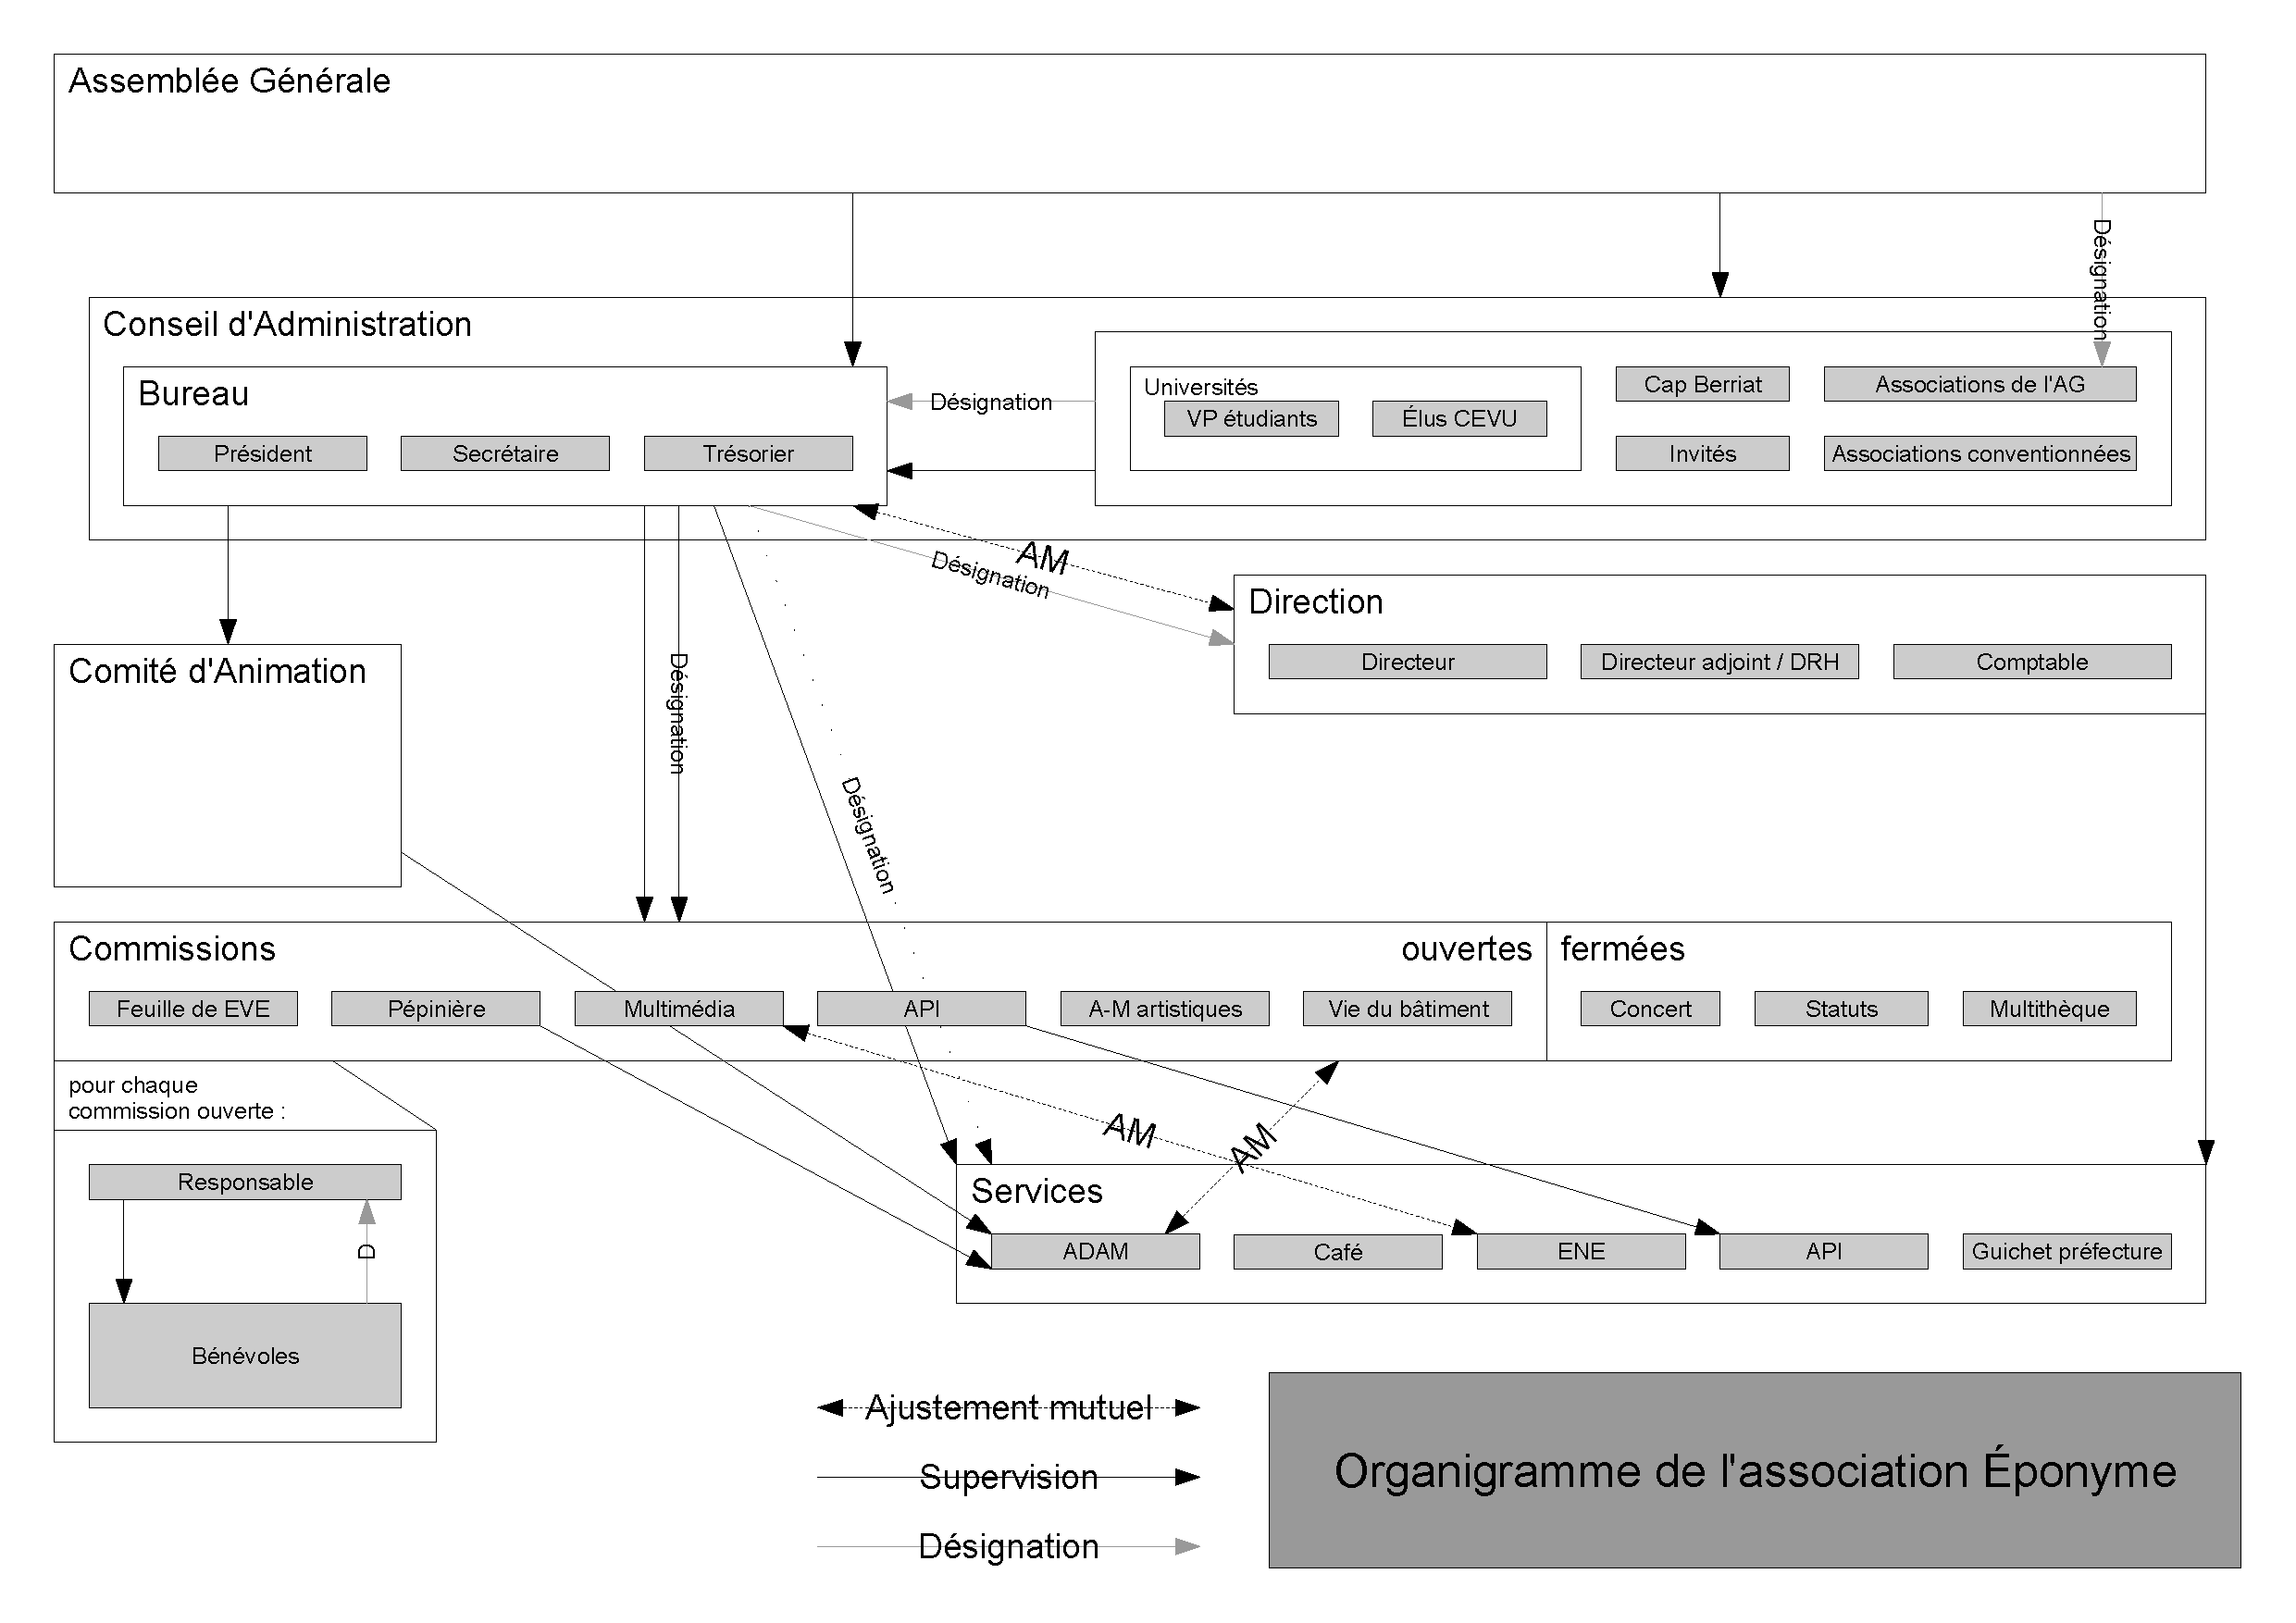
\includegraphics[trim=0mm 0mm 210mm 0mm,clip,scale=0.7]{annexes/organigramme.pdf}
\end{flushright}
\newpage
\begin{flushleft}
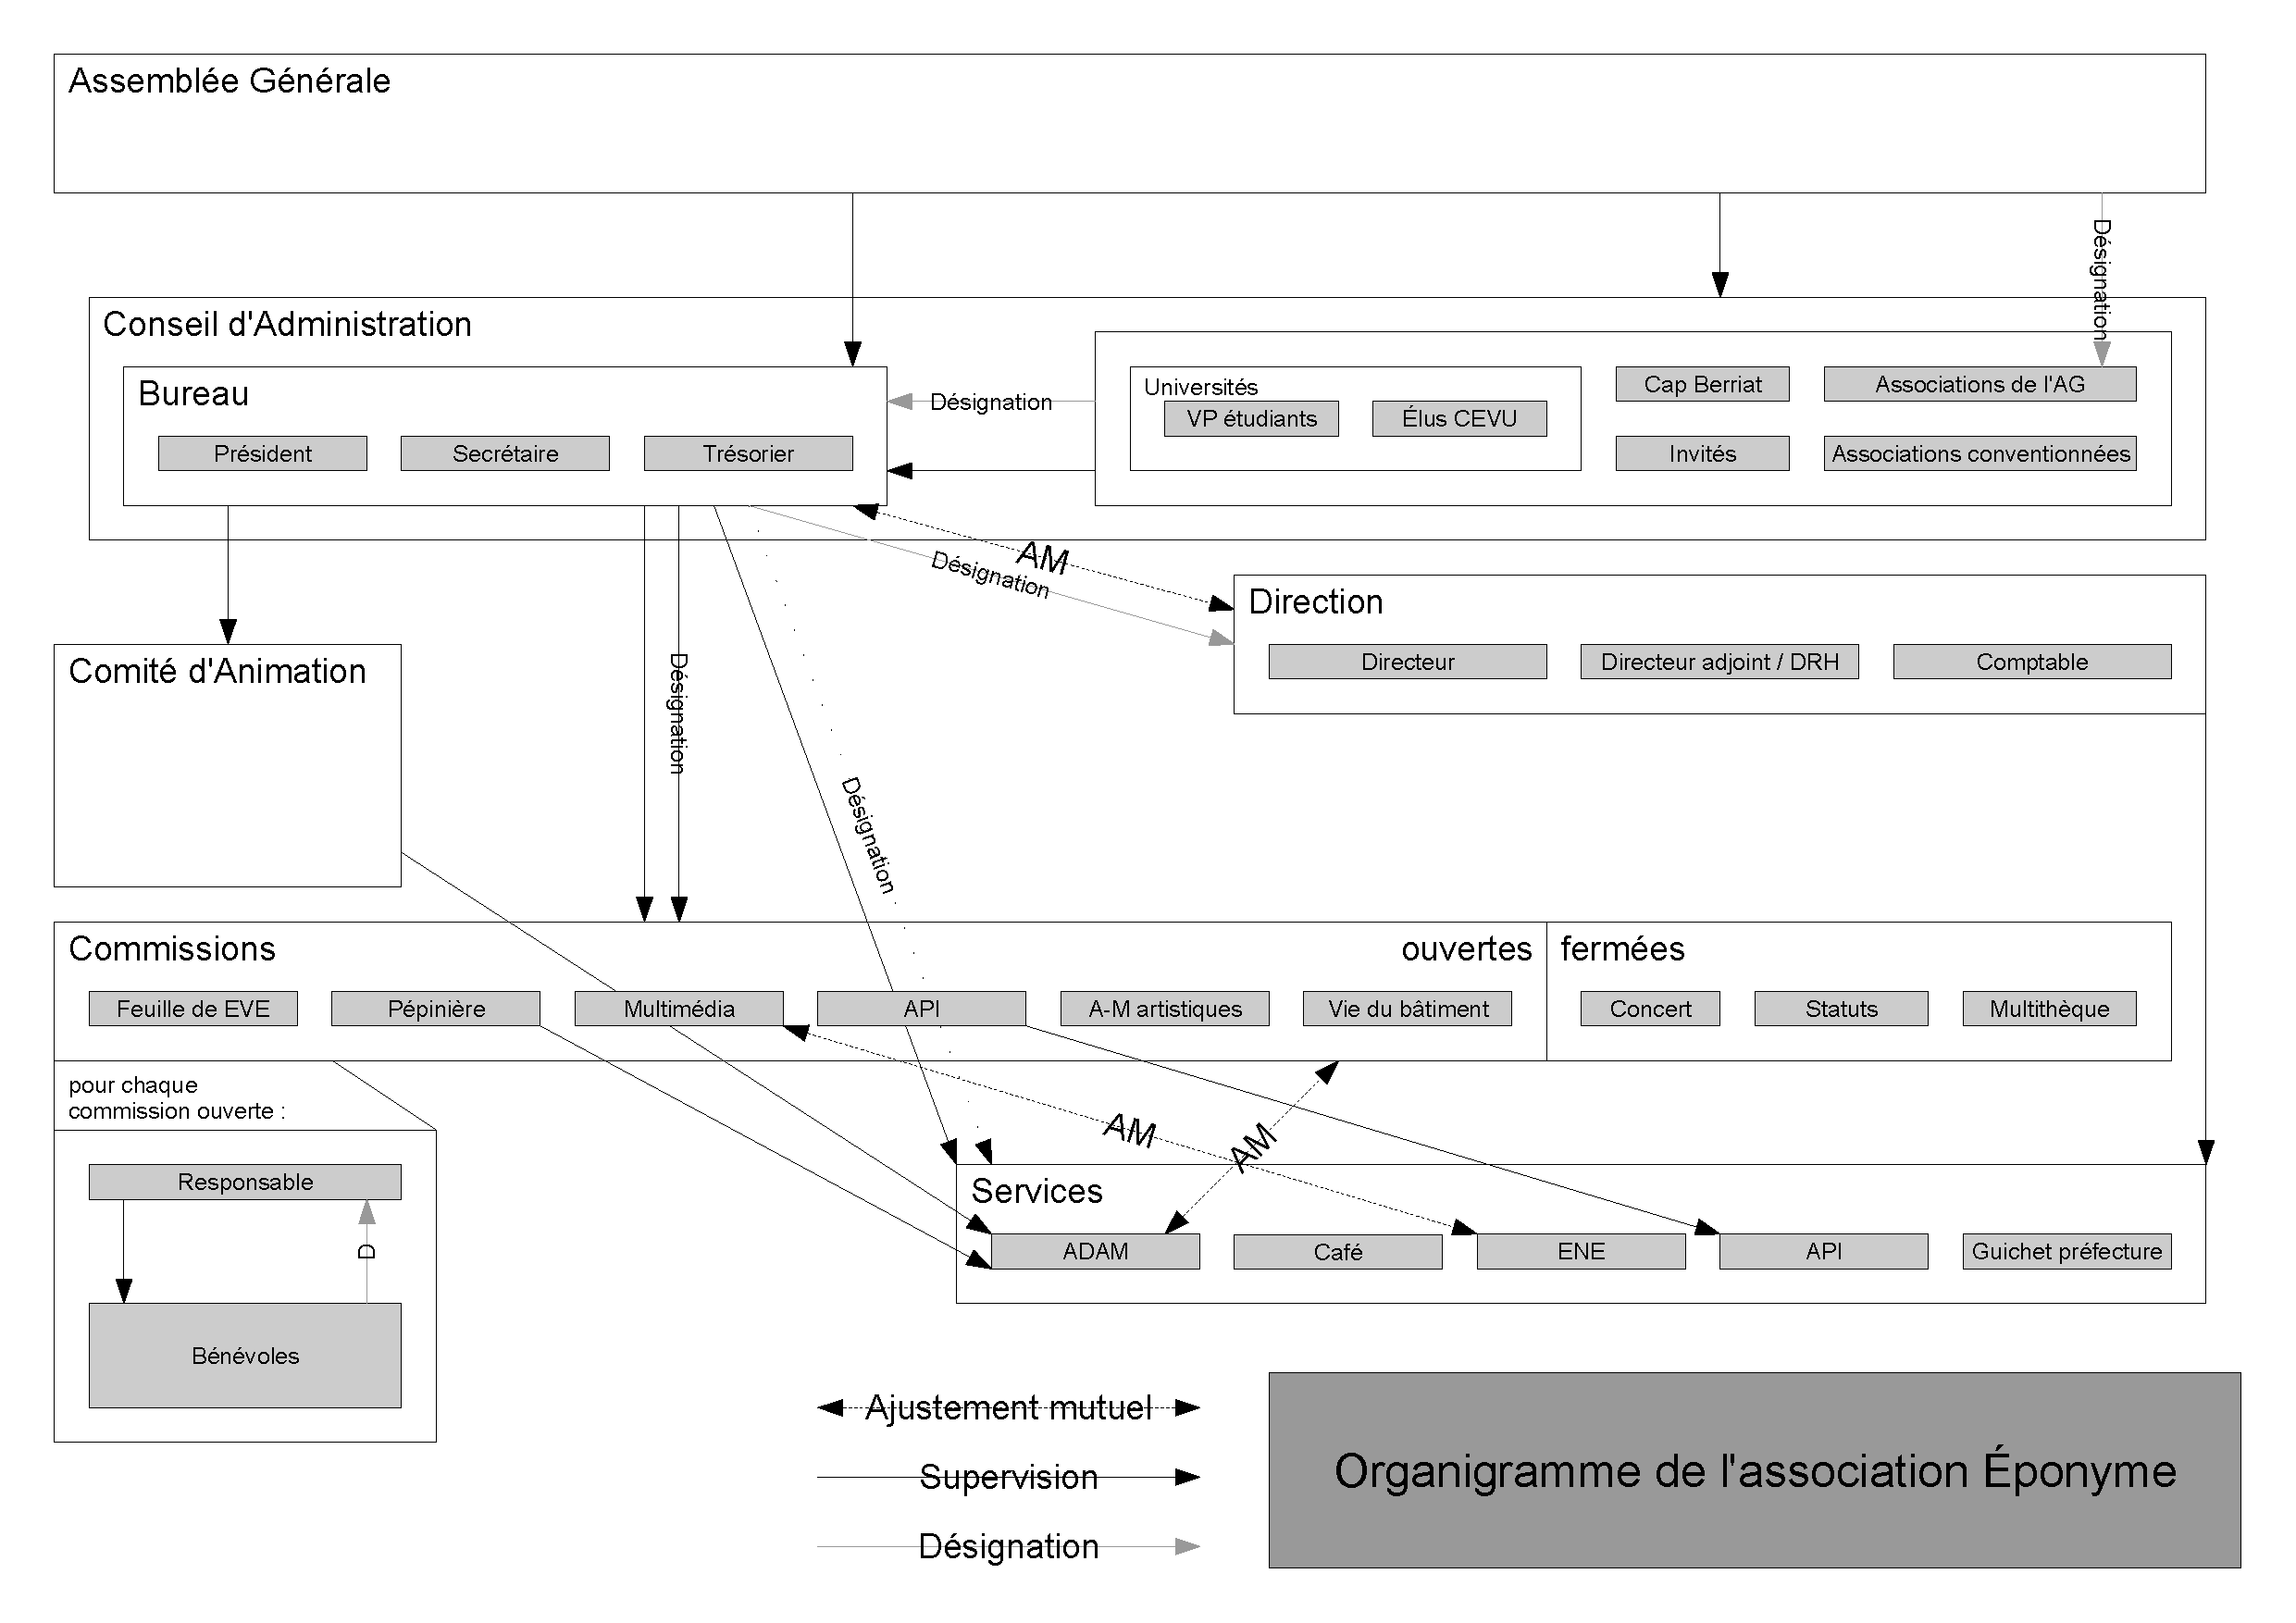
\includegraphics[trim=210mm 0mm 0mm 0mm,clip,scale=0.7]{annexes/organigramme.pdf}
\end{flushleft}
\newpage

\section{Instances de EVE}

\label{parcoursstruct}

\subsection{L'Assemblée Générale}

L'Assemblée Générale possède l'autorité absolue. Elle seule peut prendre des
décisions relevant de grands choix stratégiques. Tout changement statutaire
doit par exemple être soumis à son approbation. Ce fut le cas en 2008 pour le
changement de dénomination demandé par les Universités.

Elle réunit l'ensemble des adhérents,
et les décisions sont prises par vote.
La majorité requise et le quorum fluctuent selon le type de décision.
Pour de très nombreuses raisons,et notamment des quorums trop élevés,
des contraintes matérielles déraisonnables, les statuts ne peuvent être
convenablement appliqués.

Une Assemblée Générale Extraordinaire annuelle approuve les bilans moral et
financier présentés respectivement par le Président et le Trésorier,
et désigne 3 représentants au Conseil d'Administration.

La gestion du fonctionnement au cours de l'année et le traitement de questions
urgentes est délégué au Conseil d'Administration.

\subsection{Le Conseil d'Administration}
\label{ca}

Le Conseil d'Administration regroupe :

\begin{itemize}
\item Les Vice-Présidents Étudiants des trois universités grenobloises, de Grenoble INP et du CROUS ;
\item Un représentant par Conseil des Études et de la Vie Universitaire de ces quatre établissements d'enseignement supérieur ;
\item Un représentant de chaque association conventionnée :
	\begin{itemize}
	\item Intègre ;
	\item Radio Campus ;
	\item L'Association Ludique des Étudiants de Grenoble ;
	\item La Trace Jaune ;
	\item L'Aide Juridique Étudiante ;
	\end{itemize}
\item Cap Berriat ;
\item Trois représentants associatifs élus par l'Assemblée Générale.
\end{itemize}

Sont invités permanents :

\begin{itemize}
\item Grenoble, Université de l'Innovation ;
\item GreCO ;
\item La Métro ;
\item Les présidences des quatre établissements d'enseignement supérieur.
\end{itemize}

Il élit le Bureau en son sein et lui délègue toute son autorité pour toutes les décisions devant être prises entre ses réunions.

\subsection{Le Bureau}
\label{bureau}

Le Bureau est composé d'un Président, d'un Secrétaire et d'un Trésorier.
Il établit un contact régulier avec l'ensemble des équipes, ce qui en fait l'intermédiaire avec le CA. Il arrête l'ordre du jour et assure la tenue des réunions de l'Assemblée Générale et du Conseil d'Administration.

\subsection{COMA}

Le COMA, pour Comité d'Animation, regroupe :

\begin{itemize}
\item Les Vice-Présidents Étudiants ;
\item Les représentants associatifs ;
\item Grenoble, Université de l'Innovation ;
\item Le CROUS ;
\item Les représentants des associations conventionnées ;
\item Le responsable du service Pépinière.
\end{itemize}

Il autorise la mise à disposition de locaux et matériel aux associations
et commissions organisant des événements.

\subsection{Commissions}

Les commissions sont créées par le Bureau.
Chacune d'entre elles dispose d'un domaine de compétences spécifique :

\begin{itemize}
\item La commission Feuille de EVE publie un mensuel autour de l'association. Elle travaille
      en étroite collaboration avec le service communication.
\item La commission Pépinière réunit toutes les associations d'ADAM. Elle échange
      régulièrement avec Animafac autour des volontariats associatifs. Mutualisation
      et coordination sont au cœur de chaque réunion.
\item La commission Vie du bâtiment organise des événements dans les périodes creuses.
\item La commission Multithèque met à disposition des adhérents une cinquantaine
      de jeux de plateau, une centaine de bandes dessinées,
      et des journaux de la presse internationale.
\item Les autres commissions (voir \ref{organigramme}) portent des noms suffisamment compréhensibles.
\end{itemize}

Hormis les 3 exceptions qui suivent, elles sont ouvertes,
et élisent un responsable :

\begin{itemize}
\item La commission Concert ;
\item La commission Statuts, composée du directeur, du bureau et d'un représentant par
       association fondatrice (UNEF et Trace Jaune).
\item La commission Multithèque, composée de représentants de l'ALEG, la TJ, Intègre et Éponyme.
\end{itemize}


\subsection{Services}

\subsubsection{ADAM}

ADAM, Aide au Développement des Associations Motivées, couramment désignée
comme «~La Pépinière~», dispose de 3 salariés :
\begin{itemize}
\item Un responsable de service en CDD, actuellement Véronique Mino ;
\item Un responsable de la communication en Contrat Aidé, qui assure également l'accueil
      des associations entre 9h et 13h, actuellement Kimi Do ;
\item Un personnel en Contrat Aidé assurant l'accueil des associations entre 13h et 17h,
      actuellement Rodolfo Ripado.
\end{itemize}

Elle prend en charge le recensement des associations étudiantes, leur assistance
(dont la prodigation de conseils et l'organisation de formations mensuelles),
la mise à leur disposition et à celle des commissions des salles, d'équipement,
d'une boîte au lettre et de reprographies, la tenue des Comités d'Animation.
Elle assume toute la communication de la structure, qu'il s'agisse des contenus
du site Web, des lettres d'information électroniques pour les associations ou
les adhérents, et le programme papier.
Elle coordonne ses actions avec les autres pépinières associatives de
l'agglomération.

L'accès par les associations à la plupart de ces services requiert l'adhésion
de l'association à ADAM, pour un montant de 50 euros par année universitaire.

\subsubsection{Grand Café}

La gestion du café est assurée par des responsables associatifs, actuellement
David Rouquet (trésorier) et Laureen Bonnard-Cottet (secrétaire).
Il nécessite pour des raisons légales une comptabilité séparée,
et constitue la première et quasi-exclusive source d'autofinancement de
l'association.

Pour des raisons de flexibilité, les 13 serveurs étudiants sont employés en
contrats saisonniers de 10 mois, renouvelables une fois, et d'une quotité
hebdomadaire de 7 heures. Ils font en moyenne 3 à 4 heures supplémentaires
par semaine.

\subsubsection{ENE}

L'ENE, Espace Numérique Étudiant, dispose de l'équivalent de trois
temps pleins :
\begin{itemize}
\item Un responsable de service en CDI, actuellement Mathieu Chancel ;
\item Un informaticien en CDI, actuellement Samuel Chopin ;
\item Un équivalent temps plein consacré à l'assistance et réparti
entre huit vacataires étudiants.
\end{itemize}


Il fournit une assistance logicielle et matérielle auprès des étudiants,
mais aussi personnels dont enseignants pour leurs machines personnelles.
Il loue un parc d'une centaine d'ordinateurs portables (avec une tarification
spécifique sur critères sociaux), met à disposition des ordinateurs de prêt pour
des sites universitaires délocalisés. Il assure l'installation et la maintenance
du parc informatique, le développement des outils informatiques de EVE.

\subsubsection{API}

API est le pôle de service aux étudiants étrangers de EVE.
Il dispose d'un salarié en contrat aidé. Il édite un guide à destination des
étudiants étrangers primoarrivants et assure des permanences.

\subsubsection{Guichet Préfecture}

Le Guichet Préfecture est entièrement géré par la Préfecture et Grenoble, Université de l'Innovation.
Nous l'avons donc écarté de notre audit.

\section{Diagrammes de gestion}

\subsection{Diagrammes de flux}
\label{flux}

Nous nous contentons ici de produire trois diagrammes, les autres chaînes
rencontrées étant triviales.

\subsubsection{Chaîne de fin de stock au Grand Café}

\begin{center}
\begin{dot2tex}
digraph FinStockBar {
  size = "7!"
  rankdir = "LR"
  node [ shape = "circle", style = filled, fillcolor=lightgray ];
  SI [ shape = "octagon" ];
  F [ shape = "doublecircle" ];
  SI -> S [ label = "1" ] ;
  S -> R [ label = "2" ];
  R -> F [ label = "3" ];
  F -> S [ label = "4" ];
  S -> SI [ label = "5" ];
  S -> C [ label = "6" ];
  C -> SI [ label = "7,9" ];
  C -> F [ label = "8" ];
}
\end{dot2tex}
\end{center}
\begin{enumerate}
\item Le SI (caisse du Grand Café) indique au S (serveur) une fin de stock ;
\item S transmet l'information au responsable stocks (R) ;
\item R passe une commande au fournisseur (F) ;
\item F livre le produit, fournit un bon de livraison et une facture au S ;
\item S met à jour le stock dans le SI ;
\item S transmet le bon de livraison et la facture au comptable (C) ;
\item S saisit la facture dans le SI ;
\item S effectue le règlement (8) auprès du F ;
\item S l'indique au SI.
\end{enumerate}

\subsubsection{Adhésion d'une association à la Pépinière}

Si l'association ne souhaite qu'être référencée sur le site de EVE,
la chaîne s'interrompt à l'étape \ref{stop_point}.

\begin{center}
\begin{dot2tex}
digraph AdhesionAsso {
  size = "7!"
  rankdir = "LR"
  node [ shape = "circle", style = filled, fillcolor=lightgray ];
  A [ shape = "doublecircle" ];
  SI [ shape = "octagon" ];
  C;
  P;
  A -> SI [ label = "1" ];
  SI -> P [ label = "2" ];
  P -> SI [ label = "3,6" ];
  SI -> A [ label = "4,7,10" ];
  A -> P  [ label = "5" ];
  P -> C  [ label = "8" ];
  C -> SI [ label = "9" ];
}
\end{dot2tex}
\end{center}

\begin{enumerate}
\item L'association (A) renseigne les informations nécessaire dans le SI ;
\item Le SI transmet à la Pépinière (P) la demande d'adhésion ;
\item P accepte la publication des données de l'association dans l'annuaire ;
\item Le SI envoie un mail à A l'informant de cette décision ;
\label{stop_point}
\item A transmet par chèque le règlement à P ;
\item P renseigne dans le SI le statut «~adhérente~» de A ;
\item Le SI envoie un mail à A l'informant de cette action ;
\item P transmet le chèque à la comptabilité (C) ;
\item C enregistre le paiement dans le SI ;
\item le SI envoie à A le reçu de ce paiement.
\end{enumerate}



\subsubsection{Demande de mise à disposition de salle ou matériel}

%edge [arrowsize=3.0]

\begin{center}
\begin{dot2tex}[circo]
digraph AdhesionAsso{
	rankdir = "LR"
	size = "9!"
	node [ shape = "circle", style = filled, fillcolor=lightgray ];

	A [ shape = "doublecircle" ];
	SI [ shape = "octagon" ];
	Po [ shape = "doublecircle" ];

	A-> SI [ label = "a"] ;
	SI -> P [ label = "b" ];
	SI -> Co [ headlabel = "c" ];

	SI -> Po [ label = "d" ];
	SI -> Ca [ label = "e" ];

	SI -> I [ label = "f" ];

	P-> SI [ label = "g" ];

	SI-> A [ label = "h" ];

	SI-> C [label = "i" ];
	
	C-> SI [ label = "j" ];
	Po -> SI [ label = "k" ];
}
\end{dot2tex}
\end{center}

\begin{enumerate}
\item L'association (A) renseigne les informations nécessaires dans SI [a] ;
\item Le SI transmet la demande à la Pépinière (P) [b] ;
\item Phase de validation du dossier par P, en boucle : 
	\begin{enumerate}
	\item P transmet à A les modifications à apporter au dossier via le SI [g,h] ;
	\item A transmet à P le dossier modifié via le SI [a,b] ;
	\end{enumerate}
\item La Pépinière valide le dossier dans le SI [g] ; 
\item Le SI transmet le dossier à la Commission Animation (C) [i] ;
\item C informe le SI de sa décision [j] ;
\item
\begin{itemize}
	\item \textbf{En cas d'acceptation :}
	\begin{enumerate}
		\item Le SI informe A de la décision de C [h] ;
		\item \textbf{Si l'événement se déroule le soir} :
		\begin{enumerate}
			\item \textbf{Selon les conditions de sécurité (type d'événement, jauge) :}
			\begin{enumerate}
				\item C indique au SI le besoin d'une équipe [j] ;
				\item Le SI le transmet au comptable (Co) [c] ;
				\item Le SI transmet à Pro One (PO) les horaires [d] ;
			\end{enumerate}
			\item Le SI indique au Café (Ca) les horaires [e] ;
		\end{enumerate}
		\item \textbf{Si A indique nécessiter un ingénieur son ou lumière} :
		\begin{enumerate}
			\item Le SI en informe le ou les ingénieurs (I) [f] ;
			\item Le SI en informe Co [c] ;
		\end{enumerate}
	\end{enumerate}
	\item \textbf{En cas d'acceptation sous condition :}
	              le SI informe A de la décision de C [h]. Retour en~1 ;
	\item \textbf{En cas de refus :} le SI informe A de la décision de C [h] ;
	\item \textbf{En cas de modification (annulation, réévaluation du public attendu :}
	\begin{enumerate}
		\item A indique au SI le changement [a] ;
		\item SI envoie une alerte à P [b] ;
		\item \textbf{Si P juge que le besoin d'une équipe de sécurité évolue :}
		\begin{enumerate}
			\item P indique au SI le besoin d'une équipe [g] ;
			\item Le SI le transmet à Co [c] ;
			\item Le SI le transmet à PO [d] ;
			\item PO notifie le SI de la possibilité de changement [k] ;
			\item Le SI le transmet à Co [c] ;
			\item Le SI le transmet à P [b].
		\end{enumerate}
	\end{enumerate}

\end{itemize}
\end{enumerate}





\section{Illustration des outils}

\subsection{Gestion des incidents}
\label{gestion_incidents}
\begin{center}
	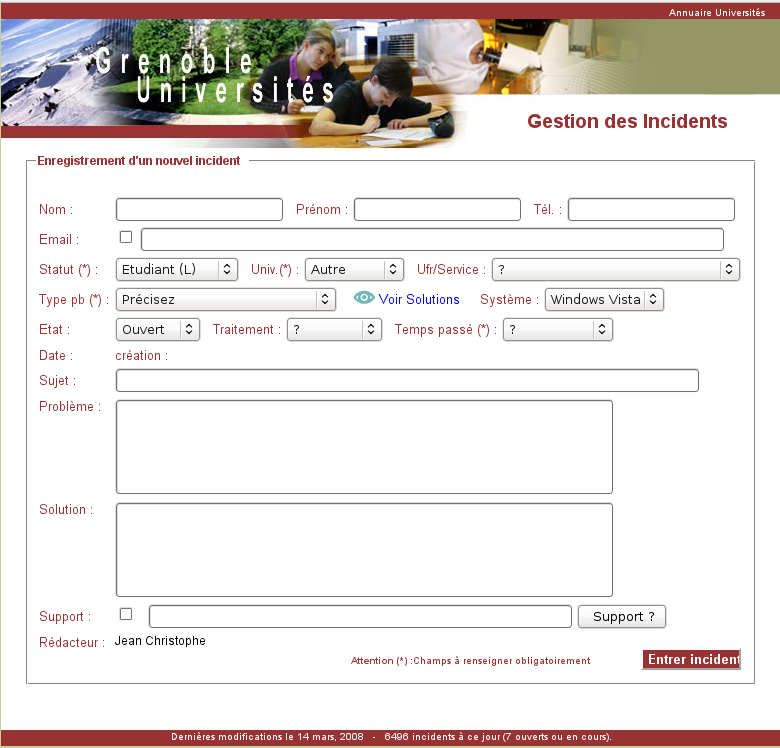
\includegraphics[width=12cm]{annexes/images/gestion_des_incidents.png} \\
	Interface de saisie des incidents de l'assistance informatique
\end{center}

\subsection{Orchestra}
\label{bar_orchestra}
\begin{center}
	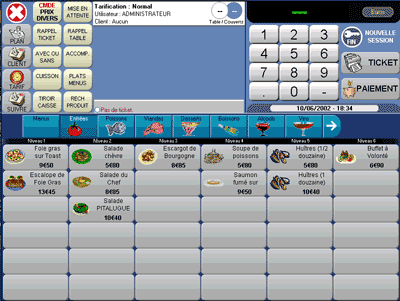
\includegraphics[width=12cm]{annexes/images/bar_orchestra.png} \\
	Interface de saisie des commandes
\end{center}

\section{Exemples de pièces}
\subsection{Extrait de bilan annuel : balance générale}
\begin{center}
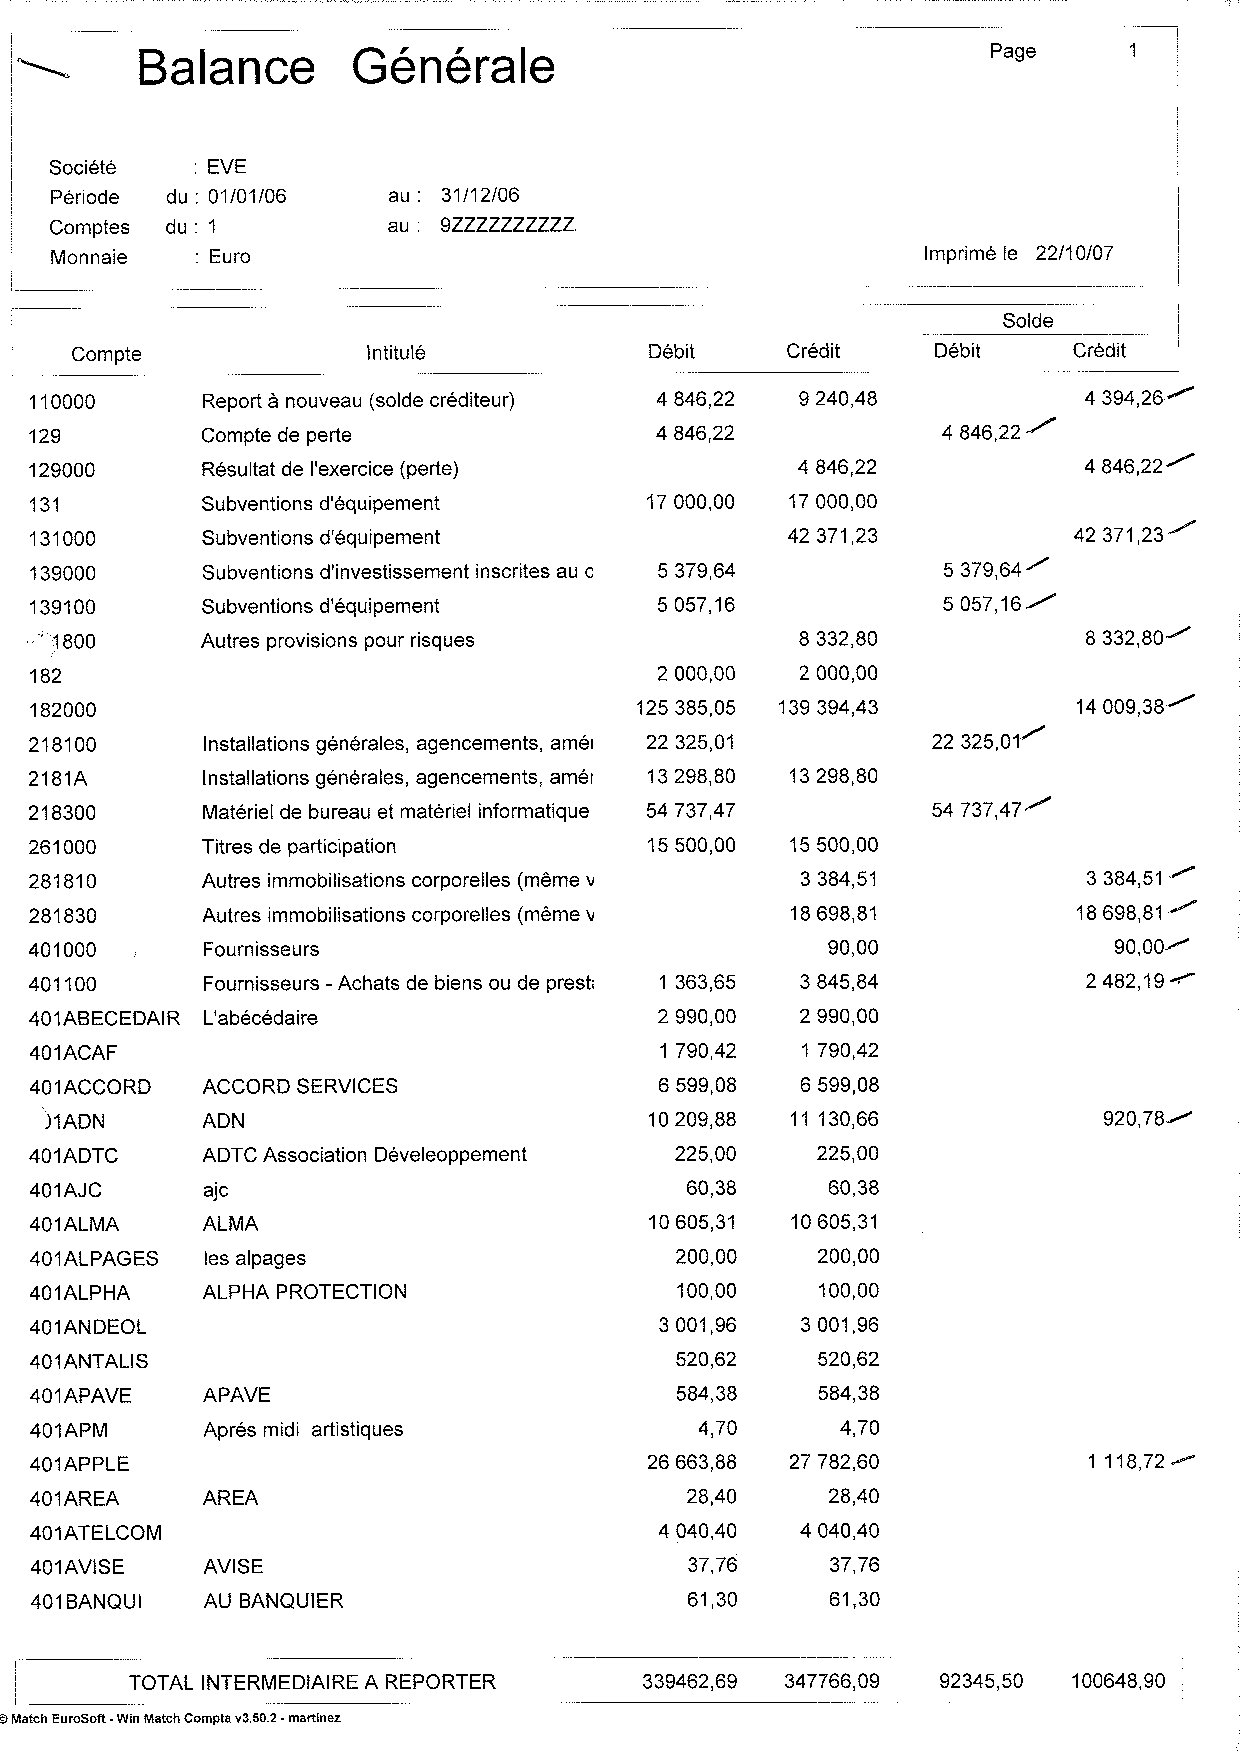
\includegraphics[height=20cm]{annexes/images/bilan_annuel_balance_generale.pdf}
\end{center}
\subsection{Extrait de bilan annuel : écritures comptables}
\begin{center}
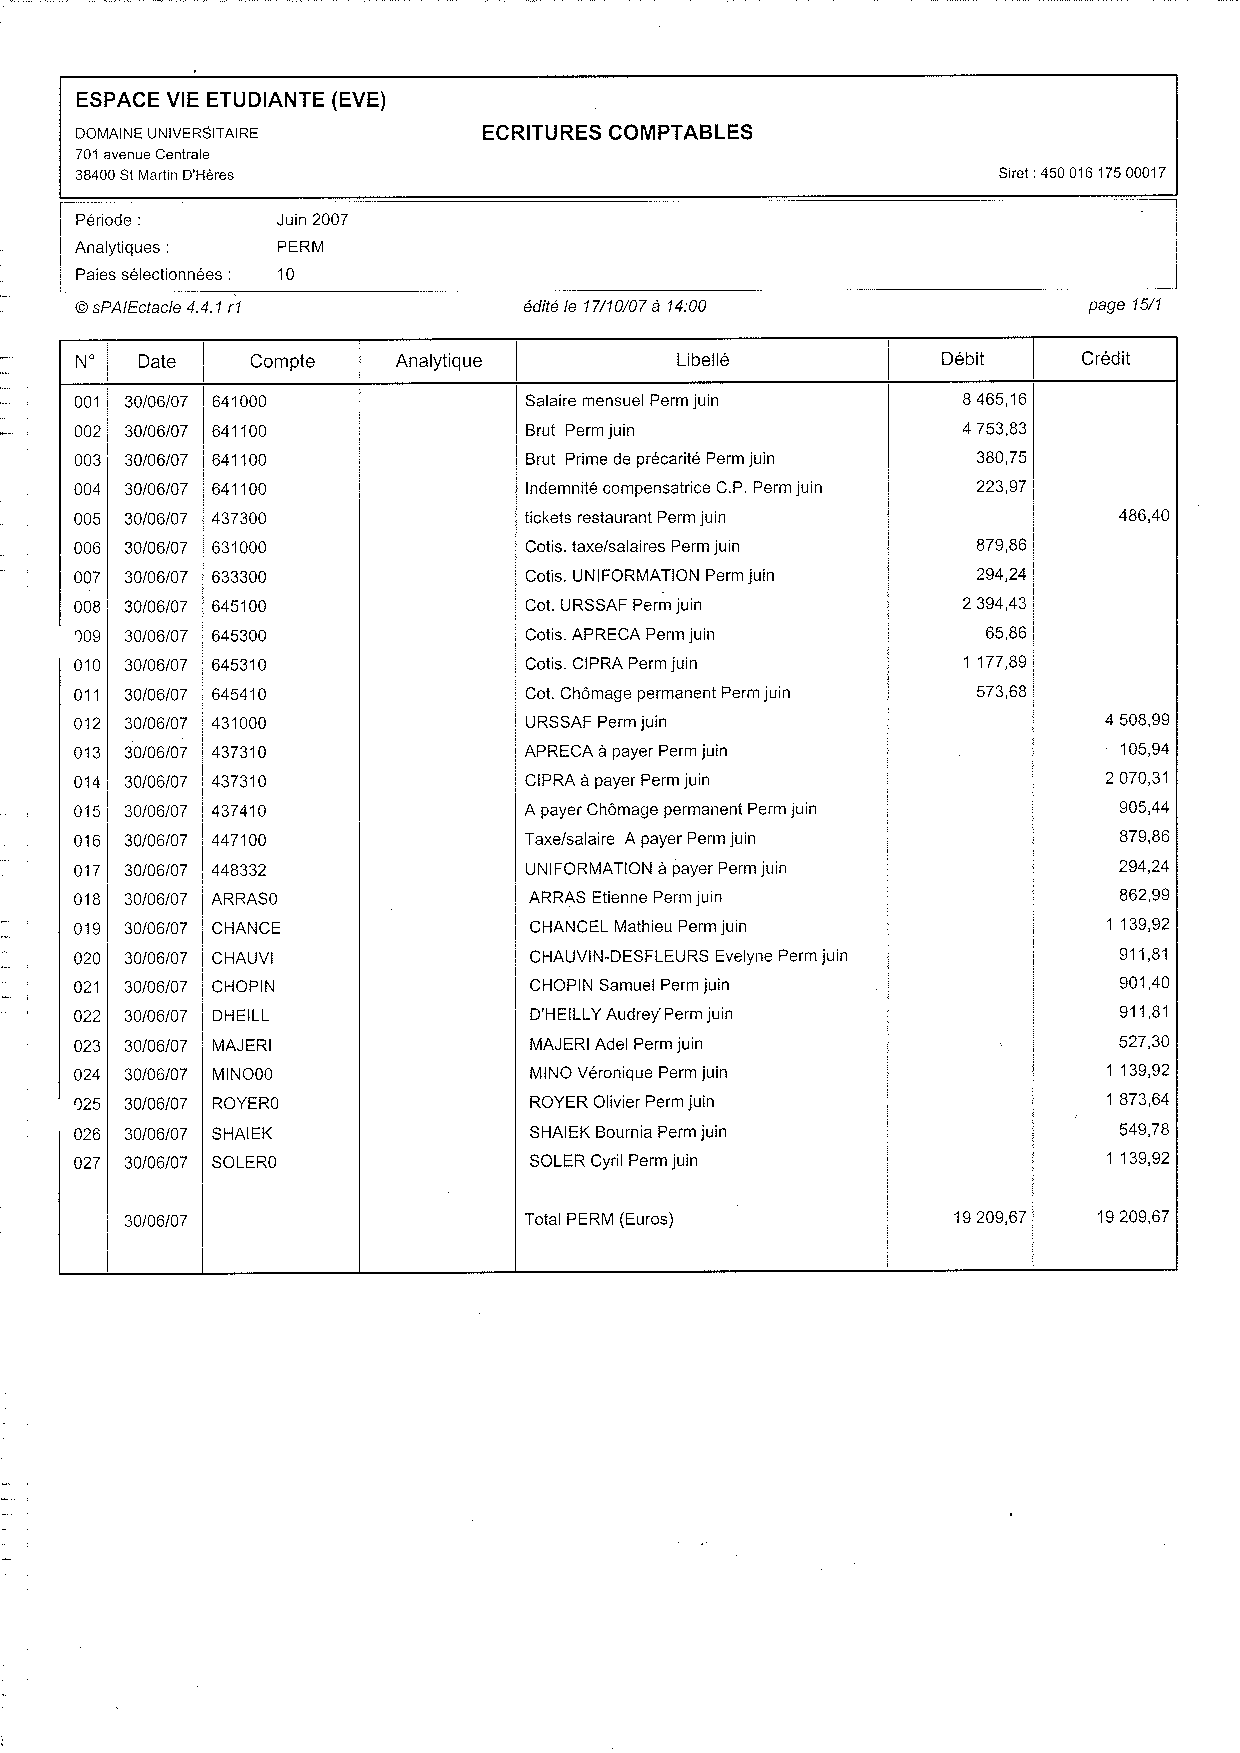
\includegraphics[height=20cm]{annexes/images/bilan_annuel_ecritures_comptables.pdf}
\end{center}
\subsection{Extrait de bilan annuel : journaux}
\begin{center}
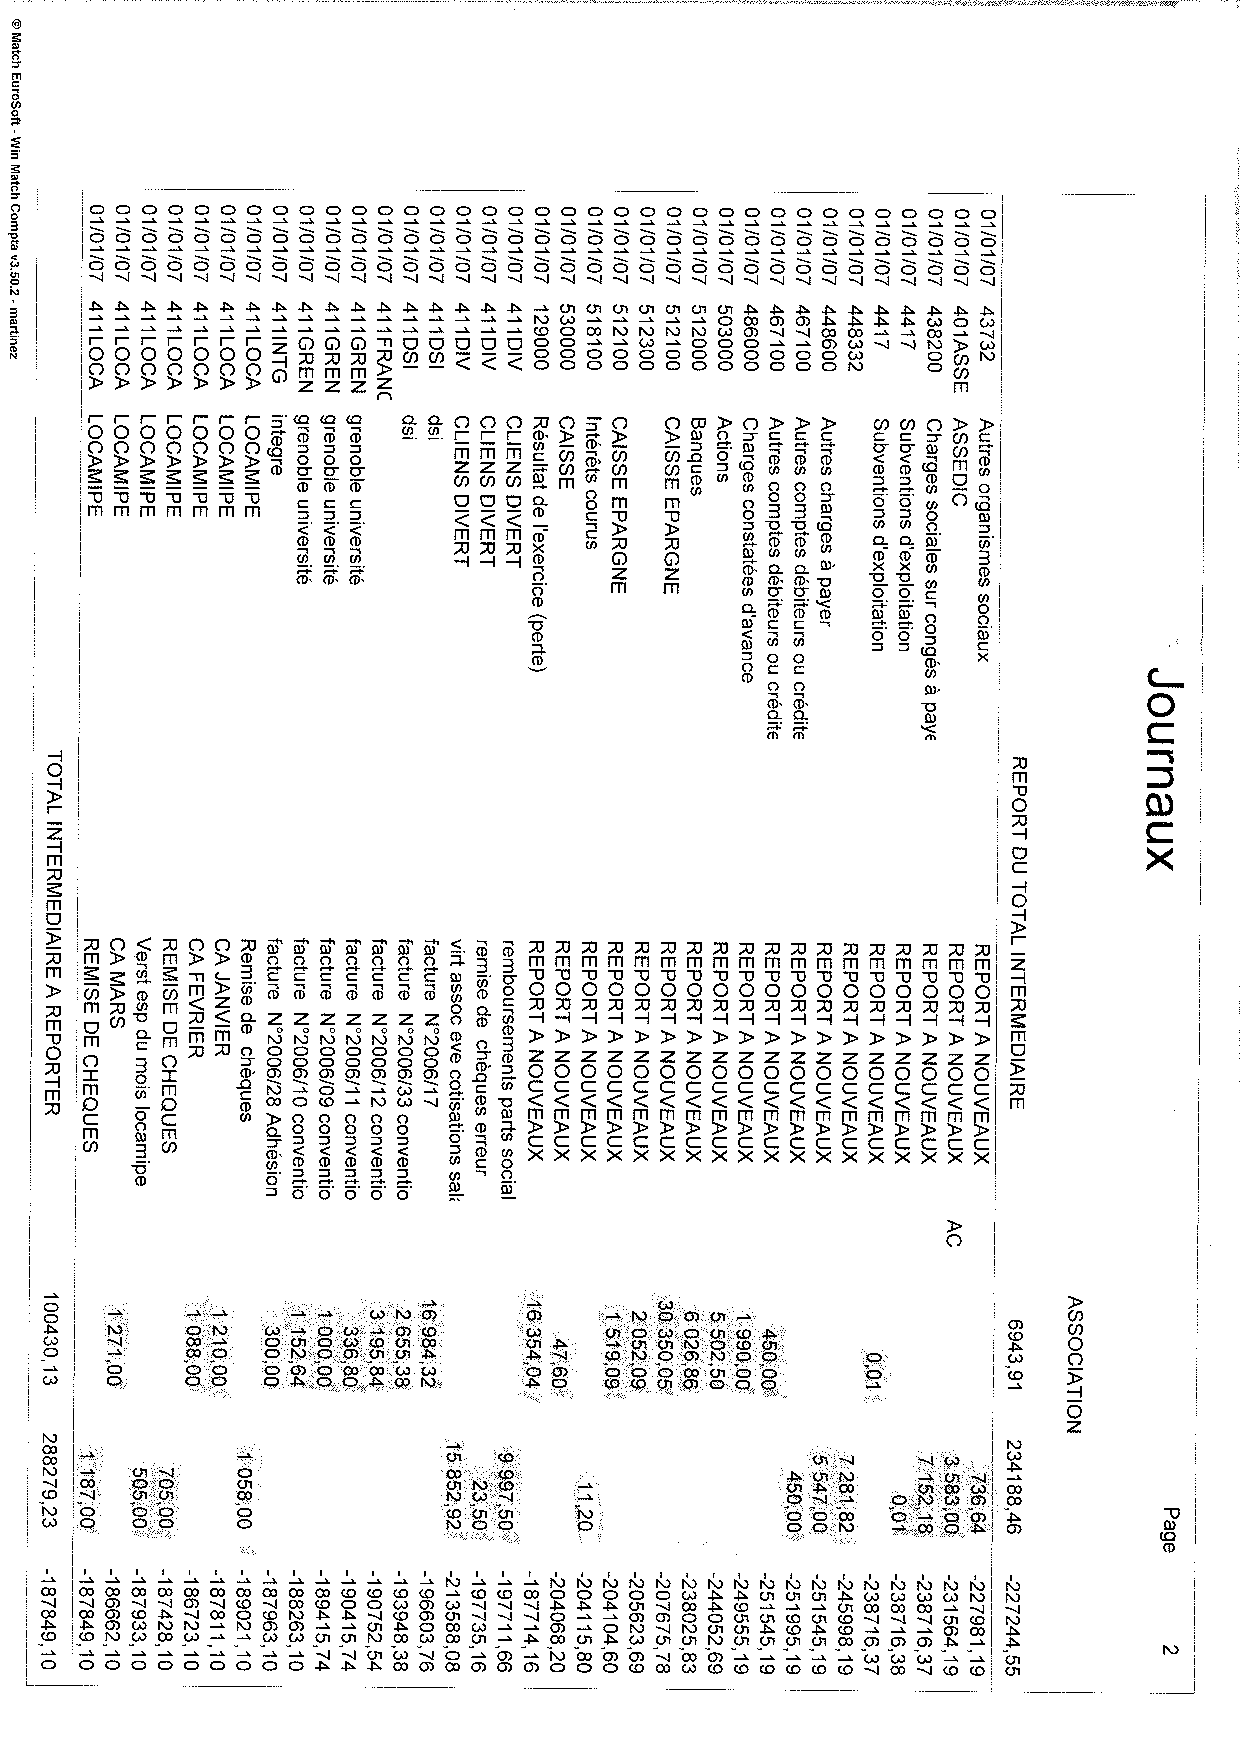
\includegraphics[scale=0.7]{annexes/images/bilan_annuel_journaux_a.pdf}
\newpage
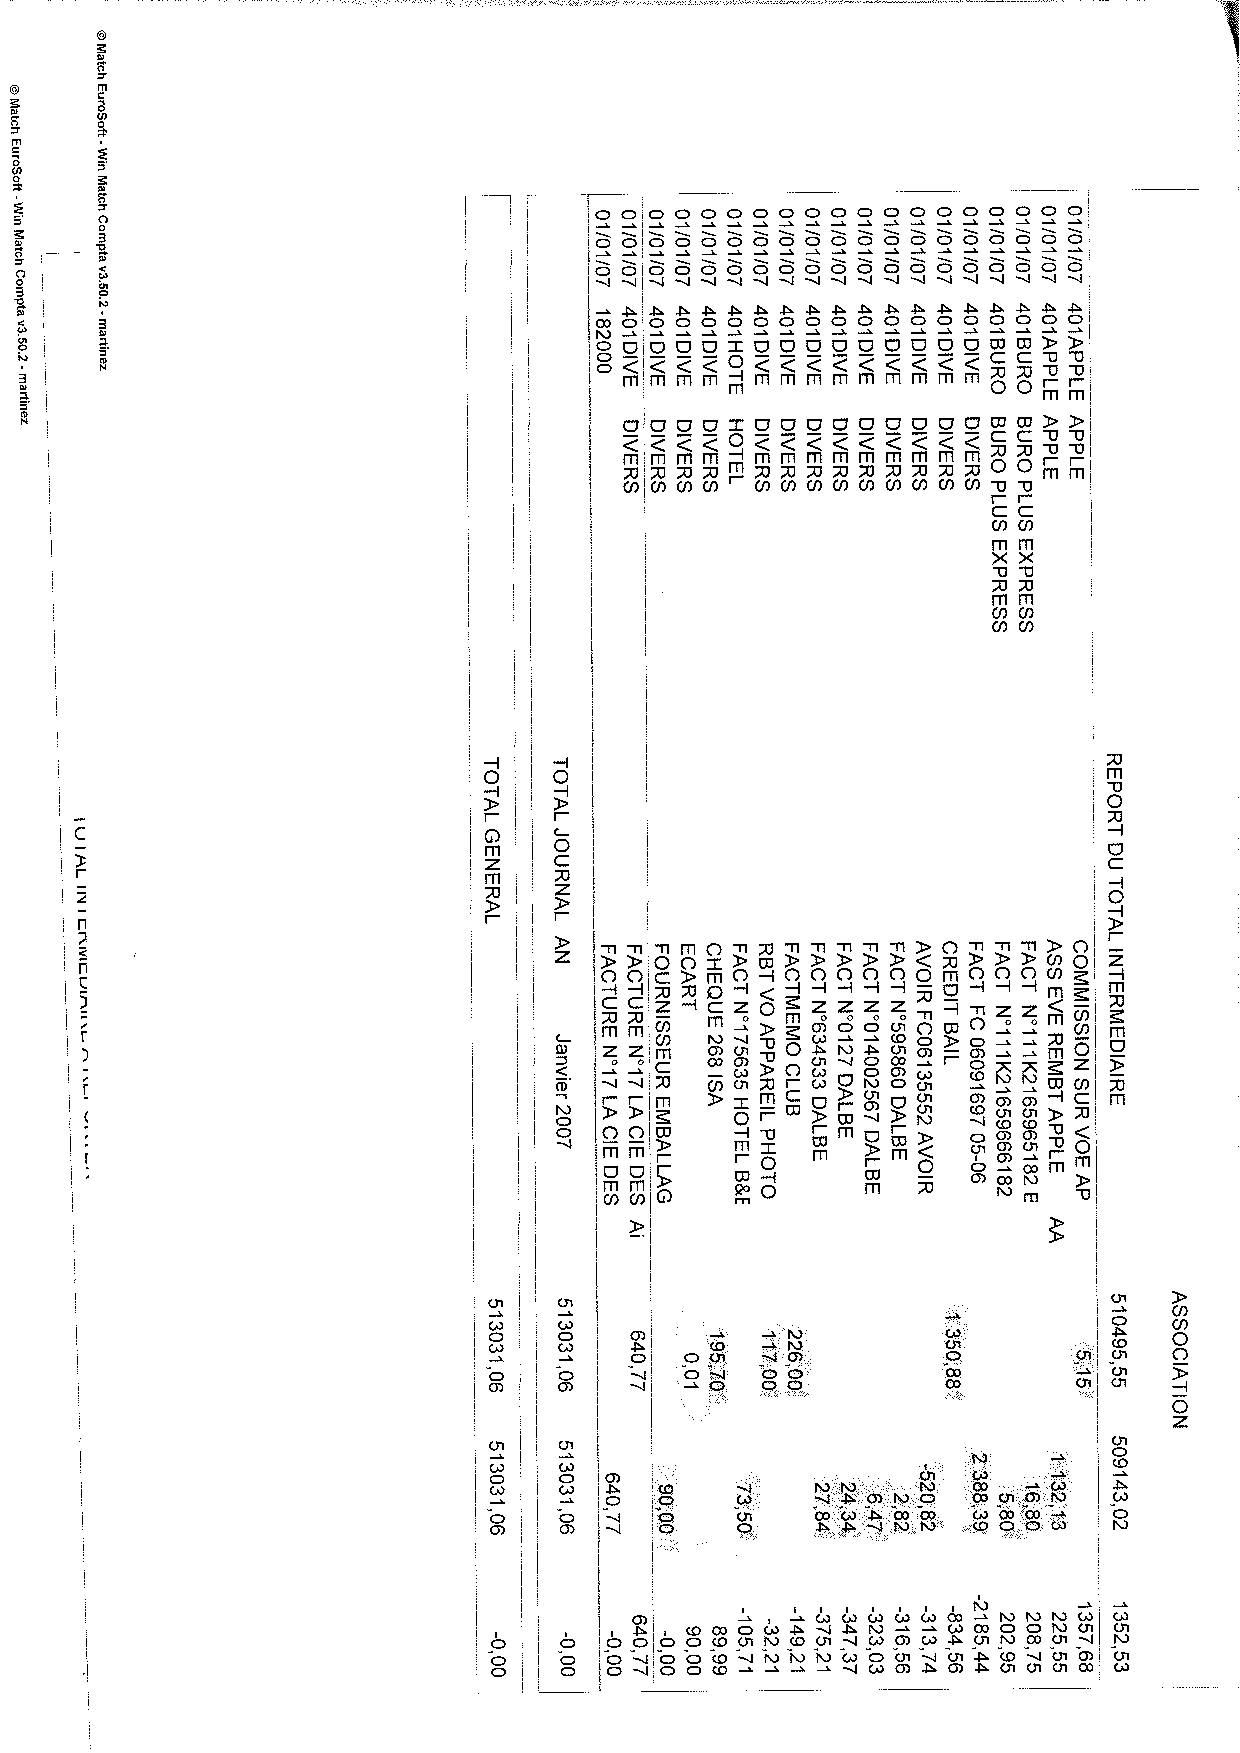
\includegraphics[scale=0.7]{annexes/images/bilan_annuel_journaux_b.pdf}
\end{center}
\subsection{Grand livre}
\begin{center}
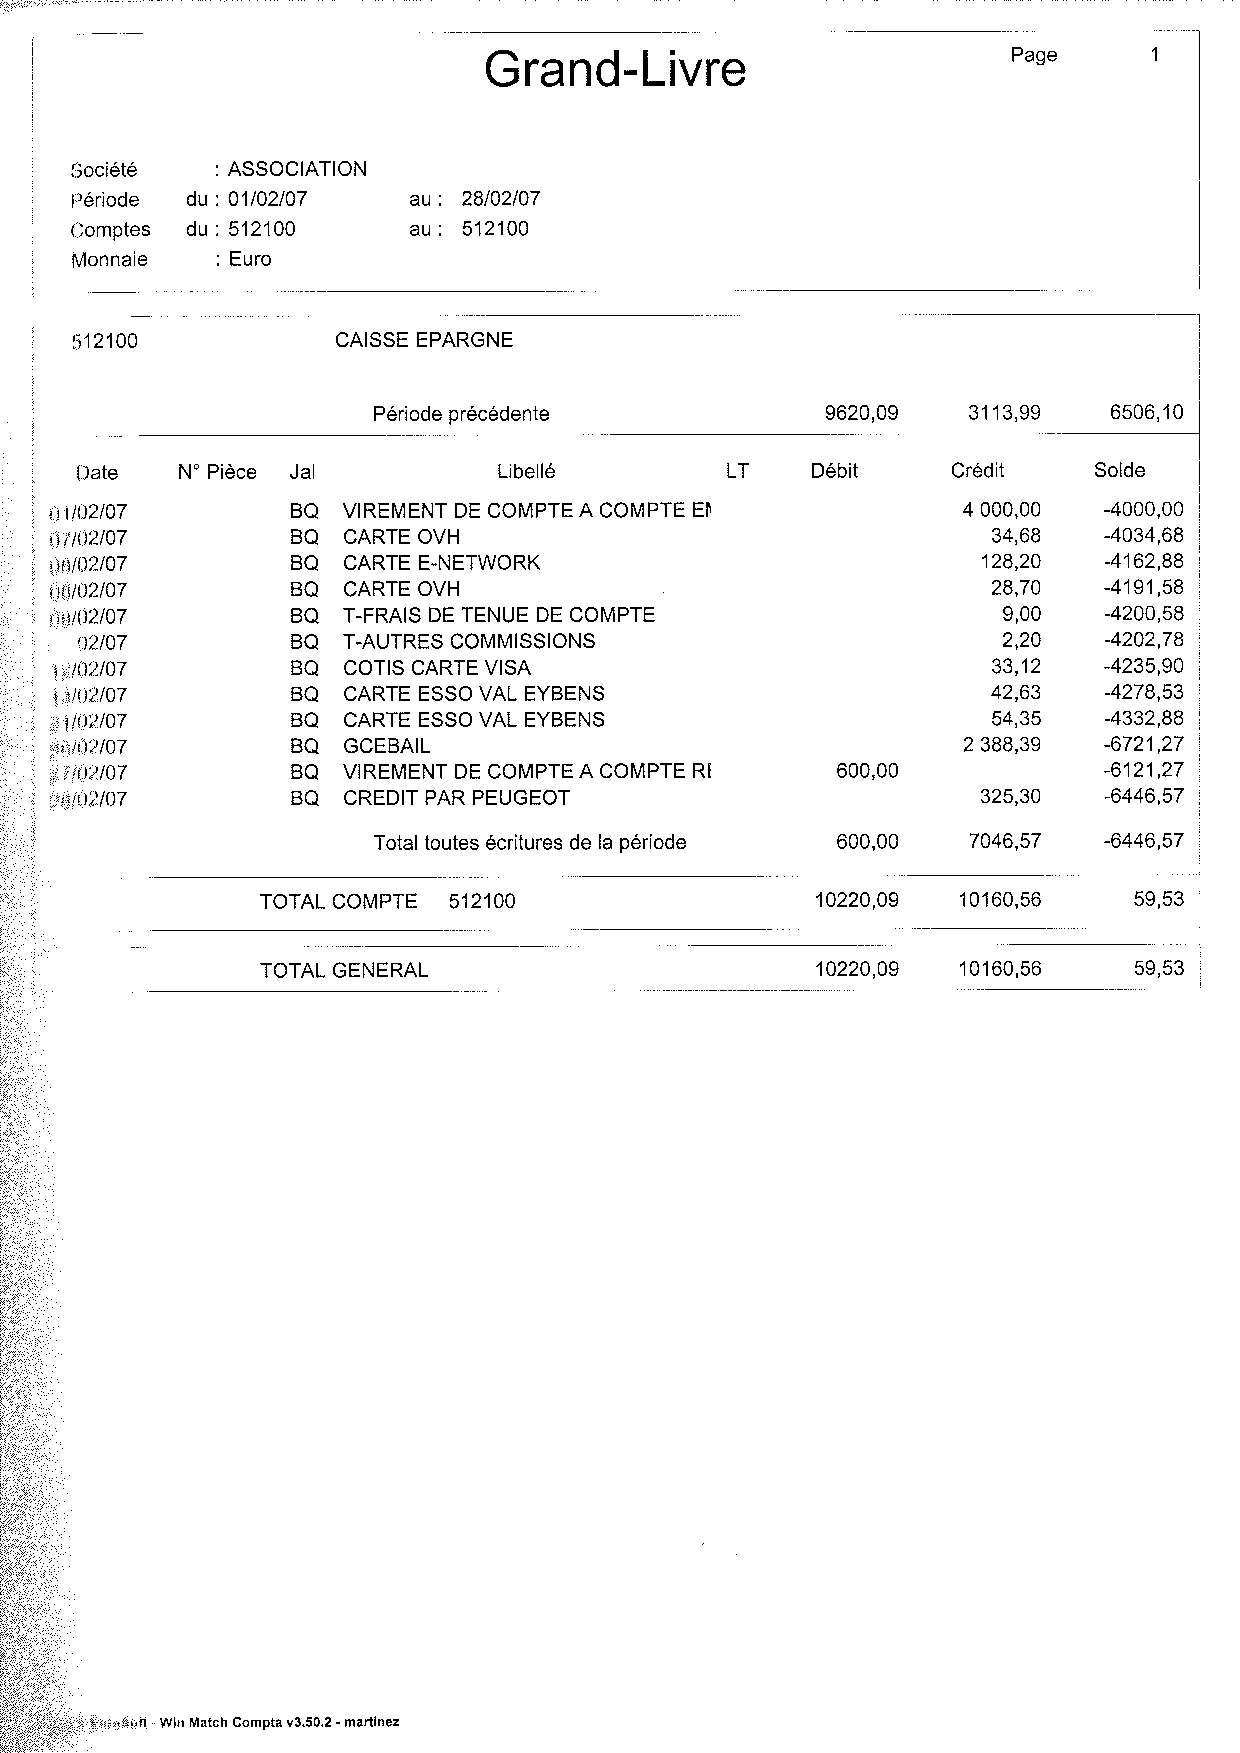
\includegraphics[height=20cm]{annexes/images/grand-livre.pdf}
\end{center}
\subsection{Avis de paiement Plan de cohésion sociale}
\begin{center}
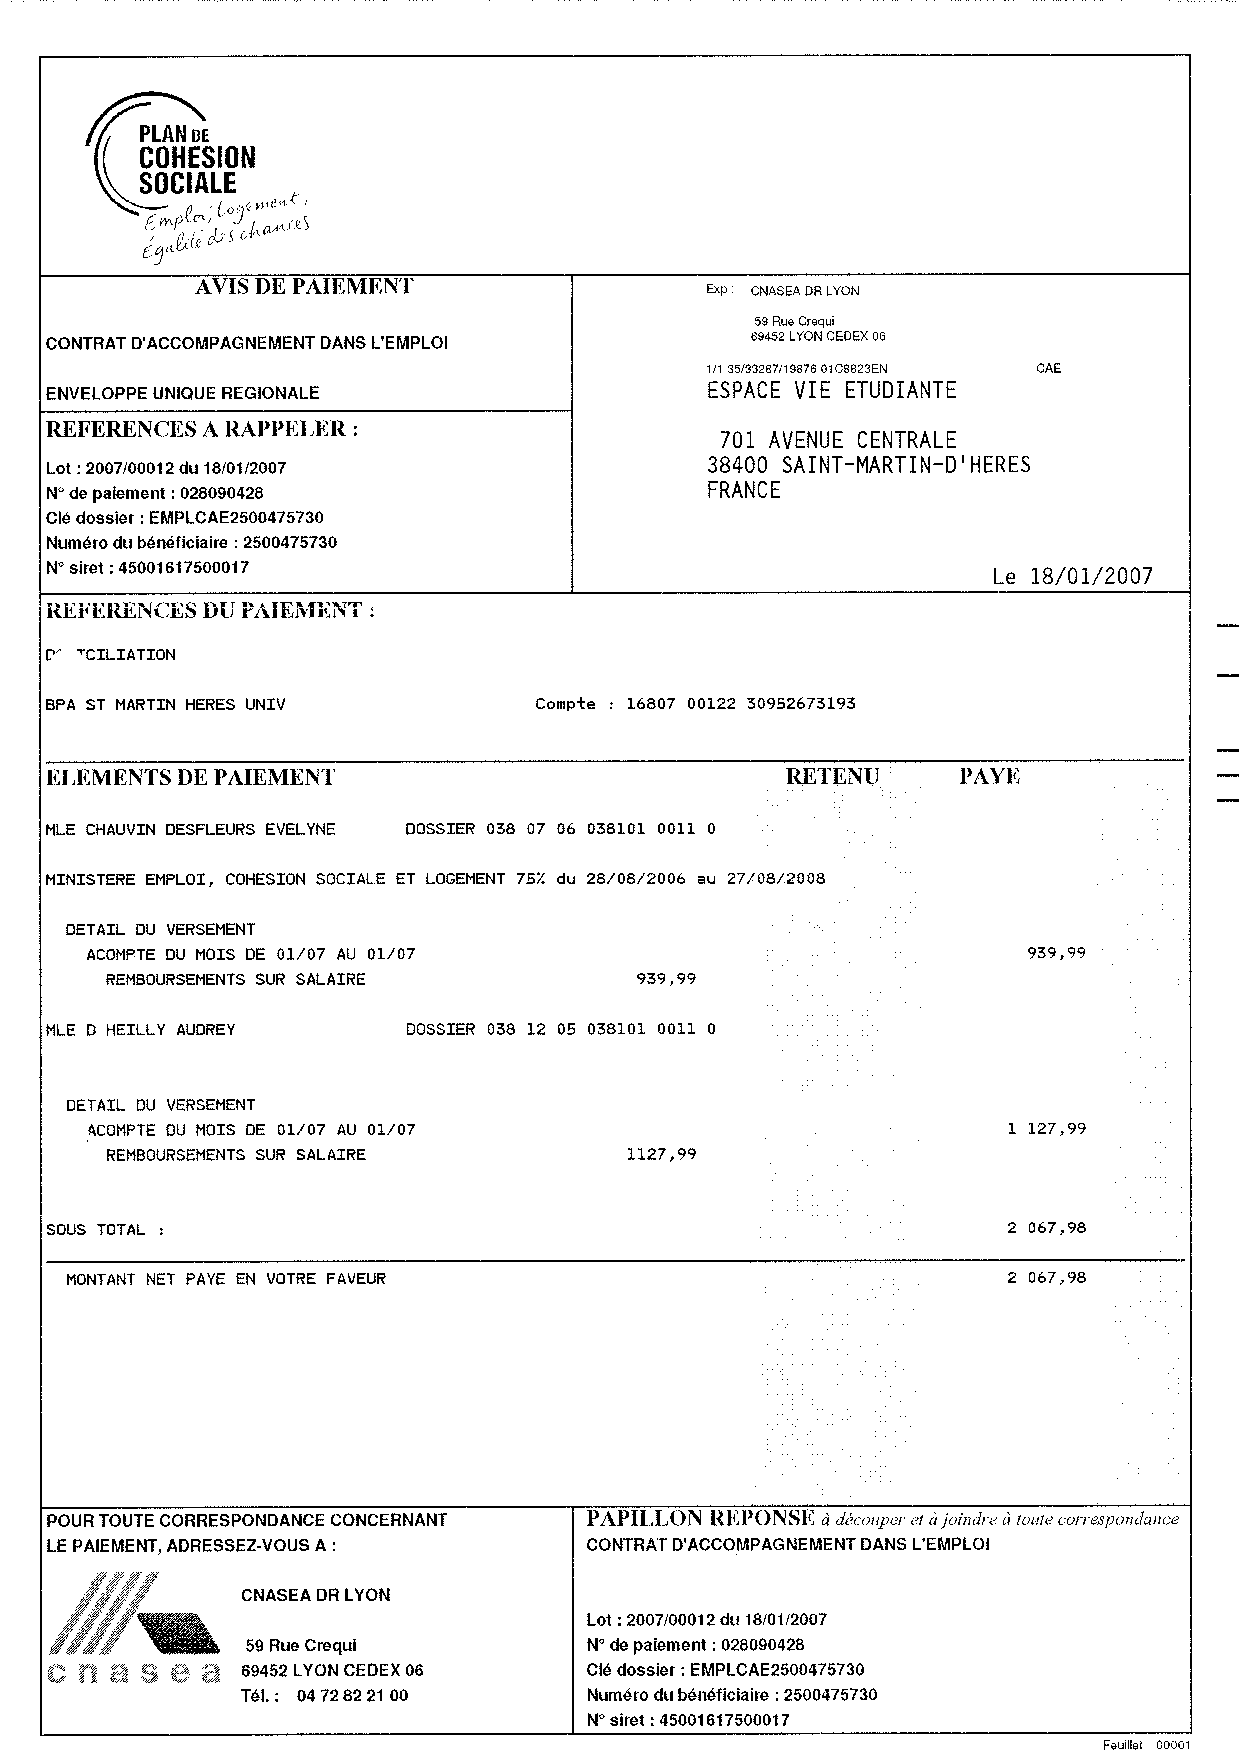
\includegraphics[scale=0.7]{annexes/images/bonne_question.pdf}
\end{center}
\subsection{Exemple de courrier rectificatif comptable}
\begin{center}
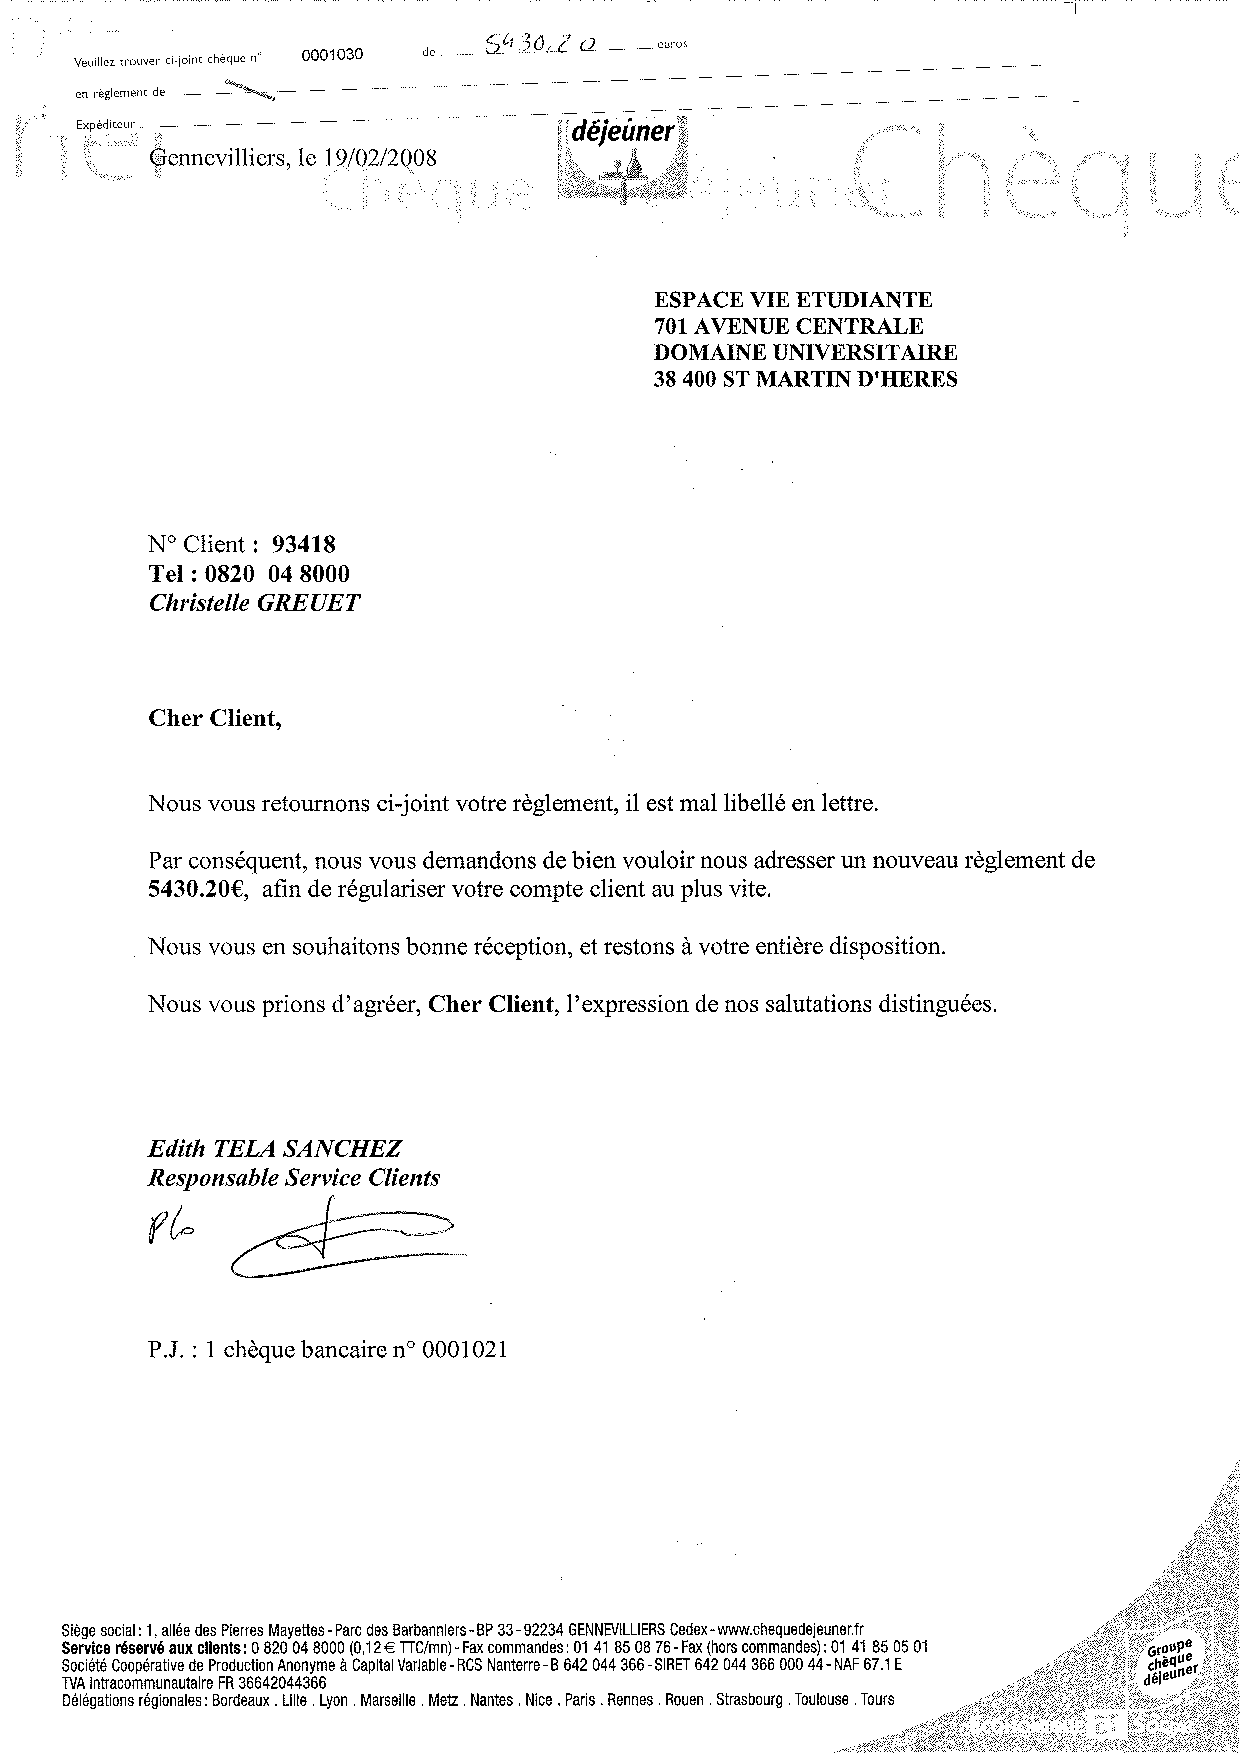
\includegraphics[scale=0.7]{annexes/images/chequedejeuner_erreur.pdf}
\end{center}
\subsection{Exemple de facture fournisseur}
\begin{center}
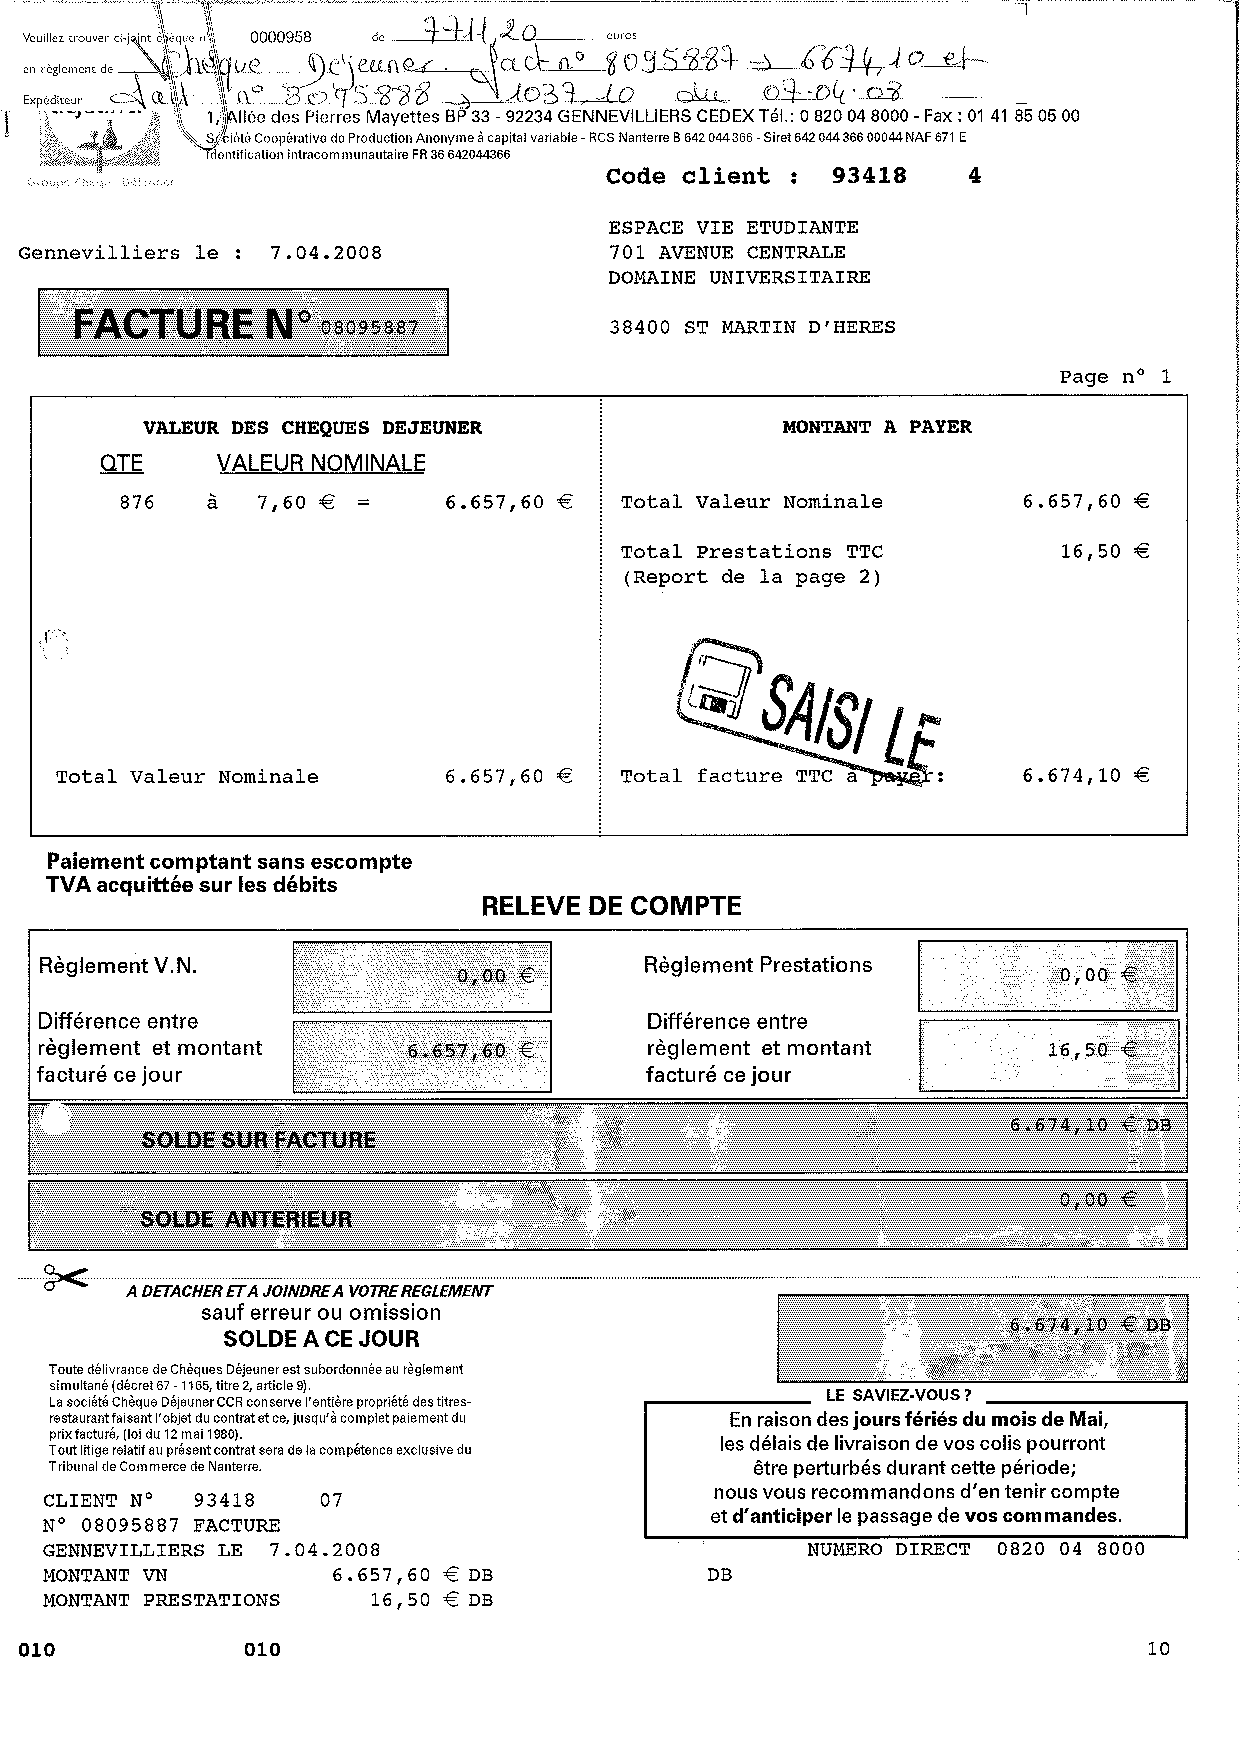
\includegraphics[scale=0.7]{annexes/images/chequedejeuner_facture.pdf}
\end{center}
\subsection{Exemple de courrier de rappel comptable}
\begin{center}
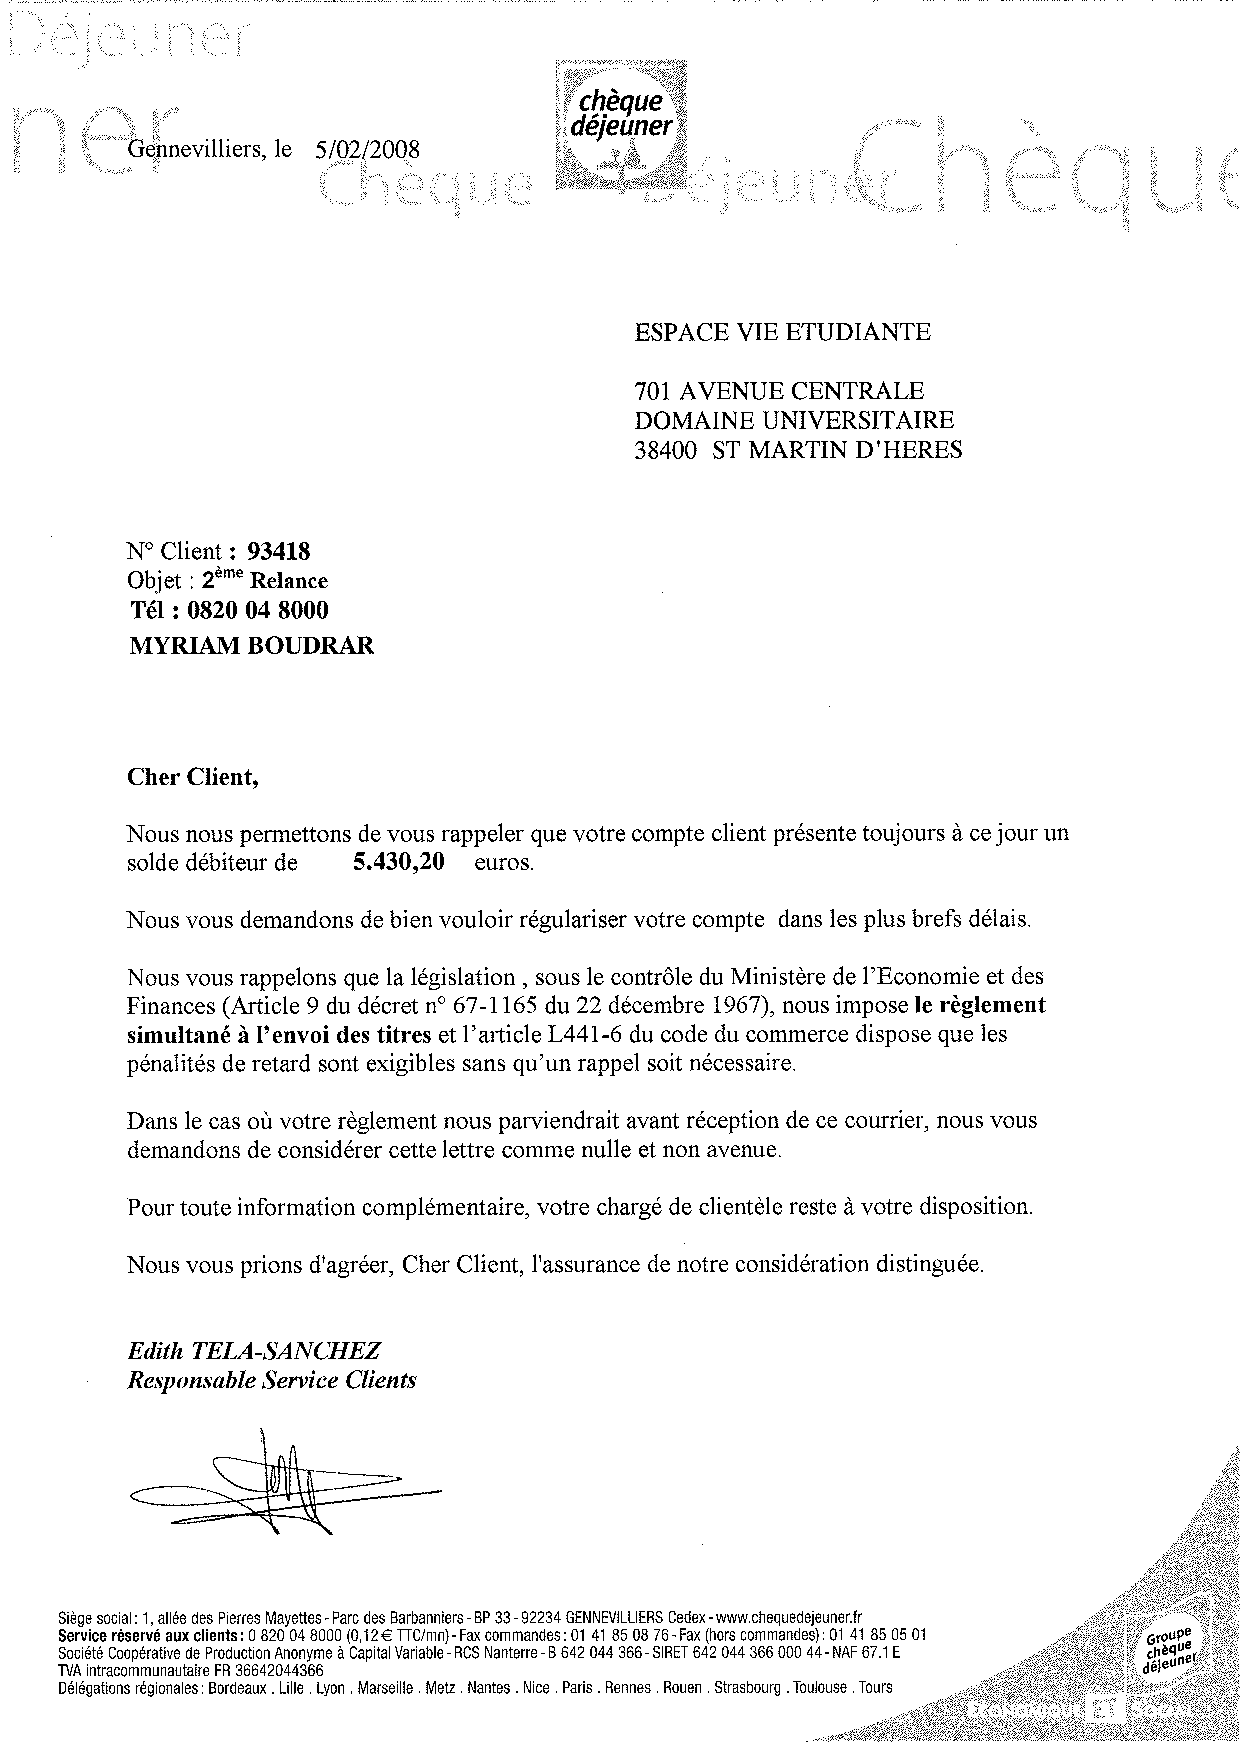
\includegraphics[scale=0.7]{annexes/images/chequedejeuner_rappel.pdf}
\end{center}
\subsection{Historique des comptes}
\begin{center}
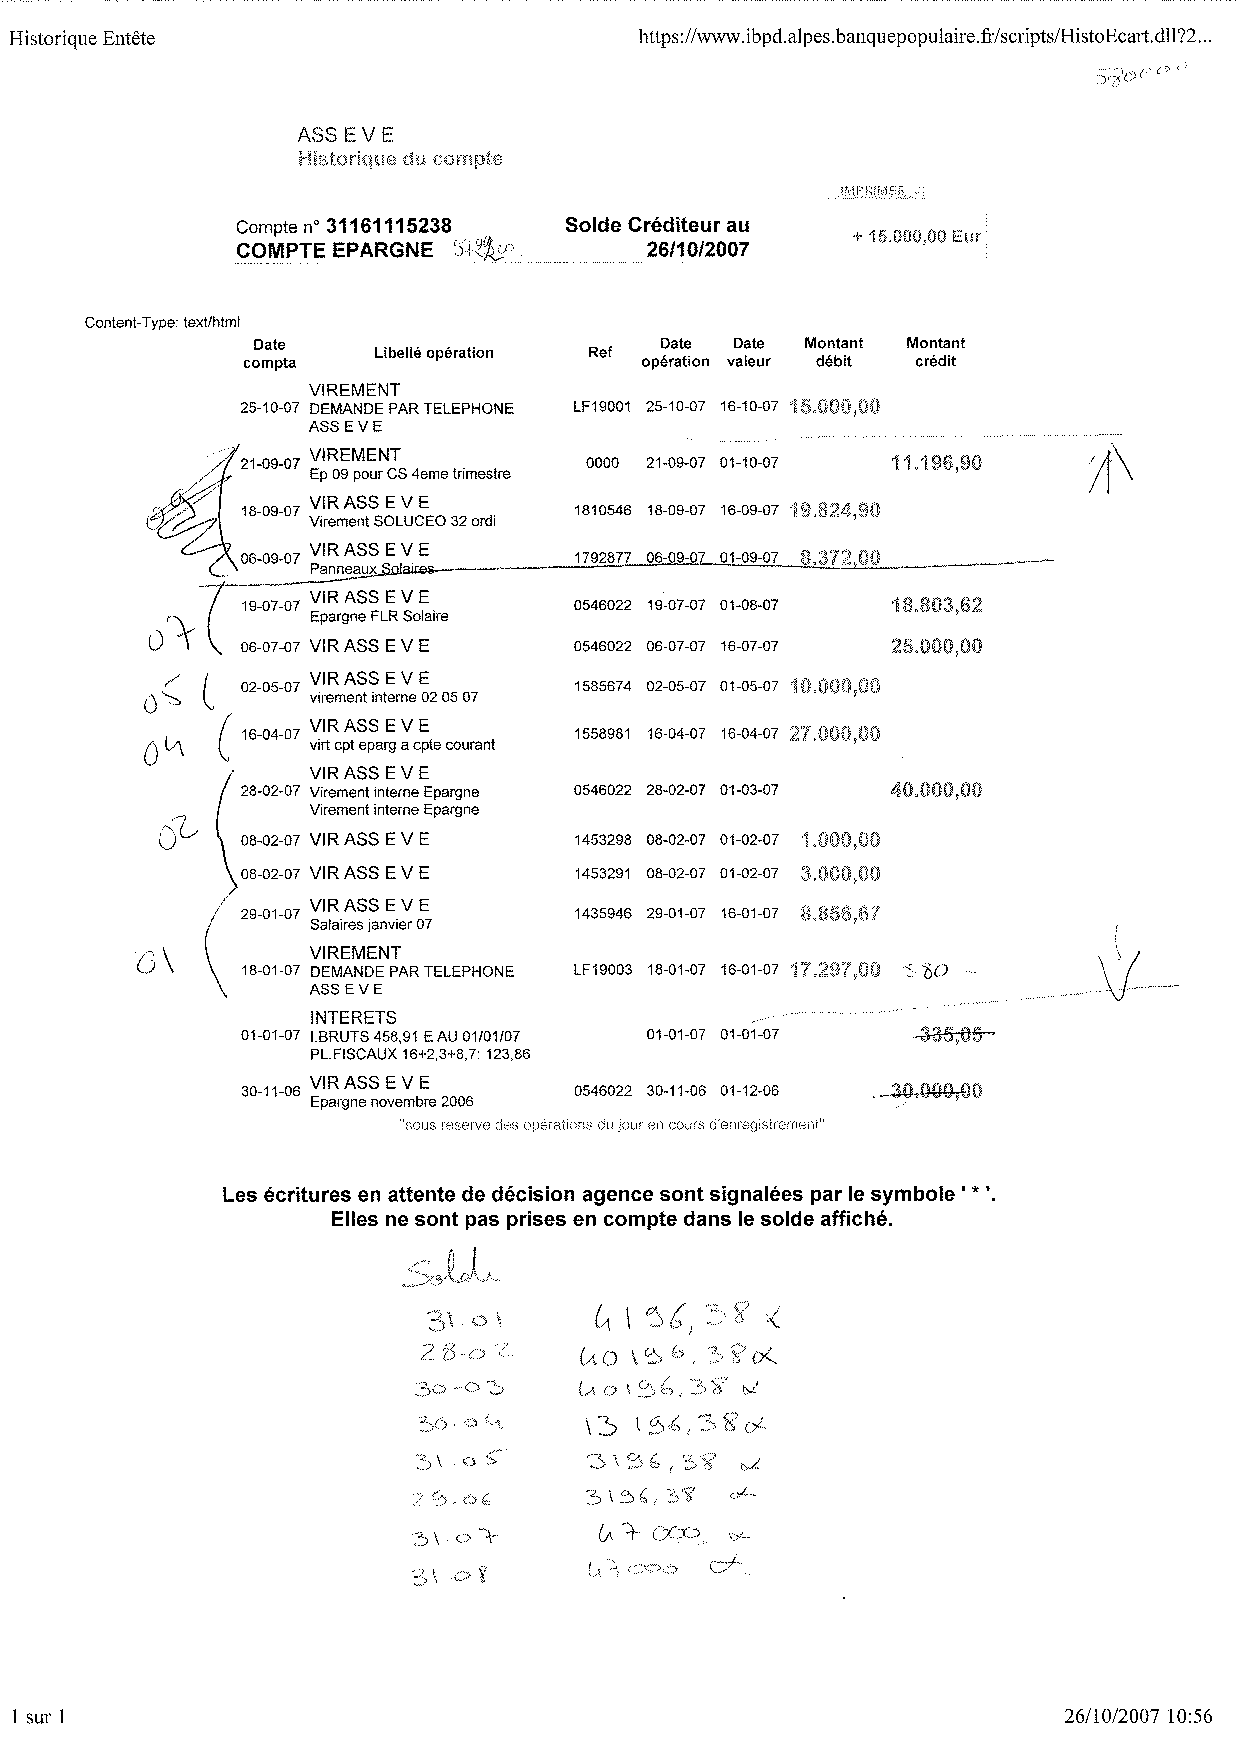
\includegraphics[scale=0.7]{annexes/images/historique_compte.pdf}
\end{center}
\subsection{Rapprochement bancaire}
\begin{center}
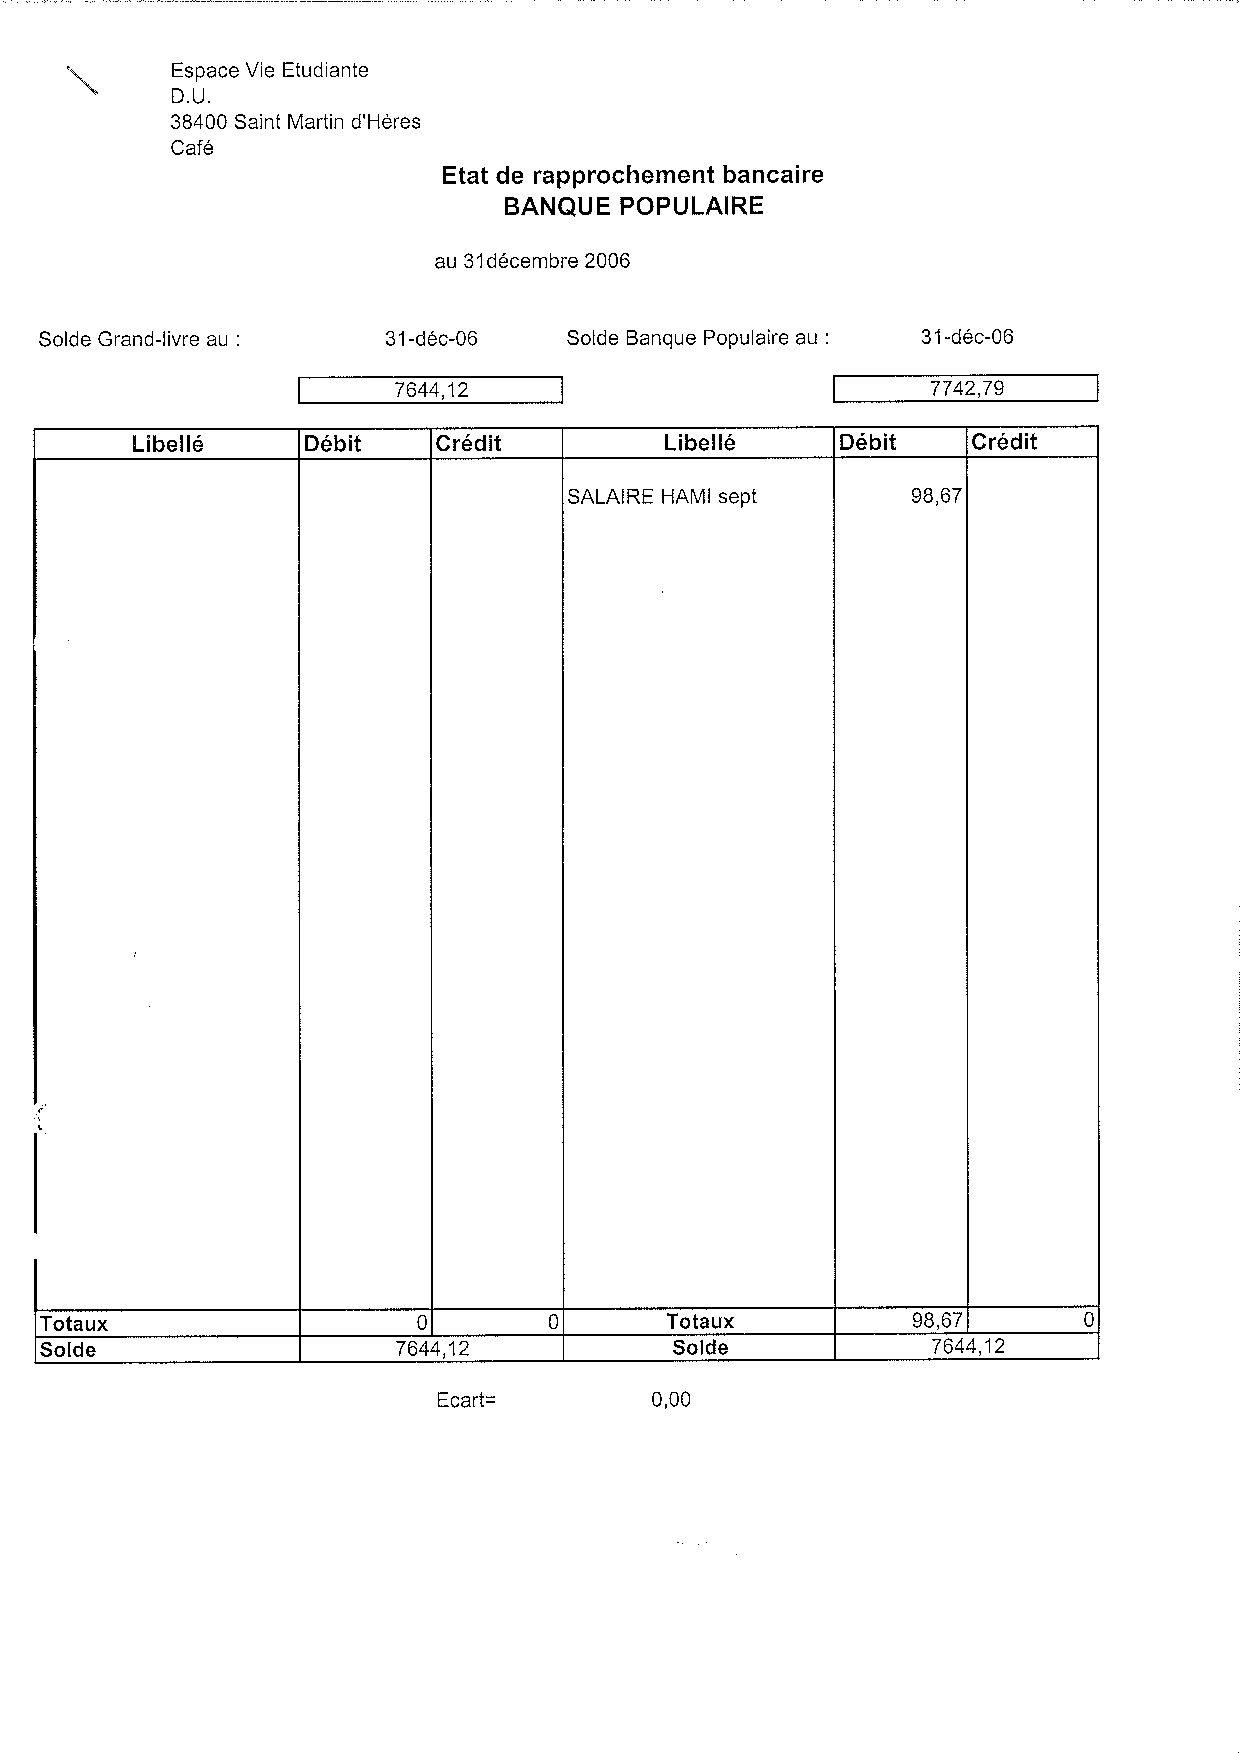
\includegraphics[scale=0.7]{annexes/images/rapprochement_bancaire.pdf}
\end{center}
\subsection{Pièce nécessitant un ajustement comptable}
\begin{center}
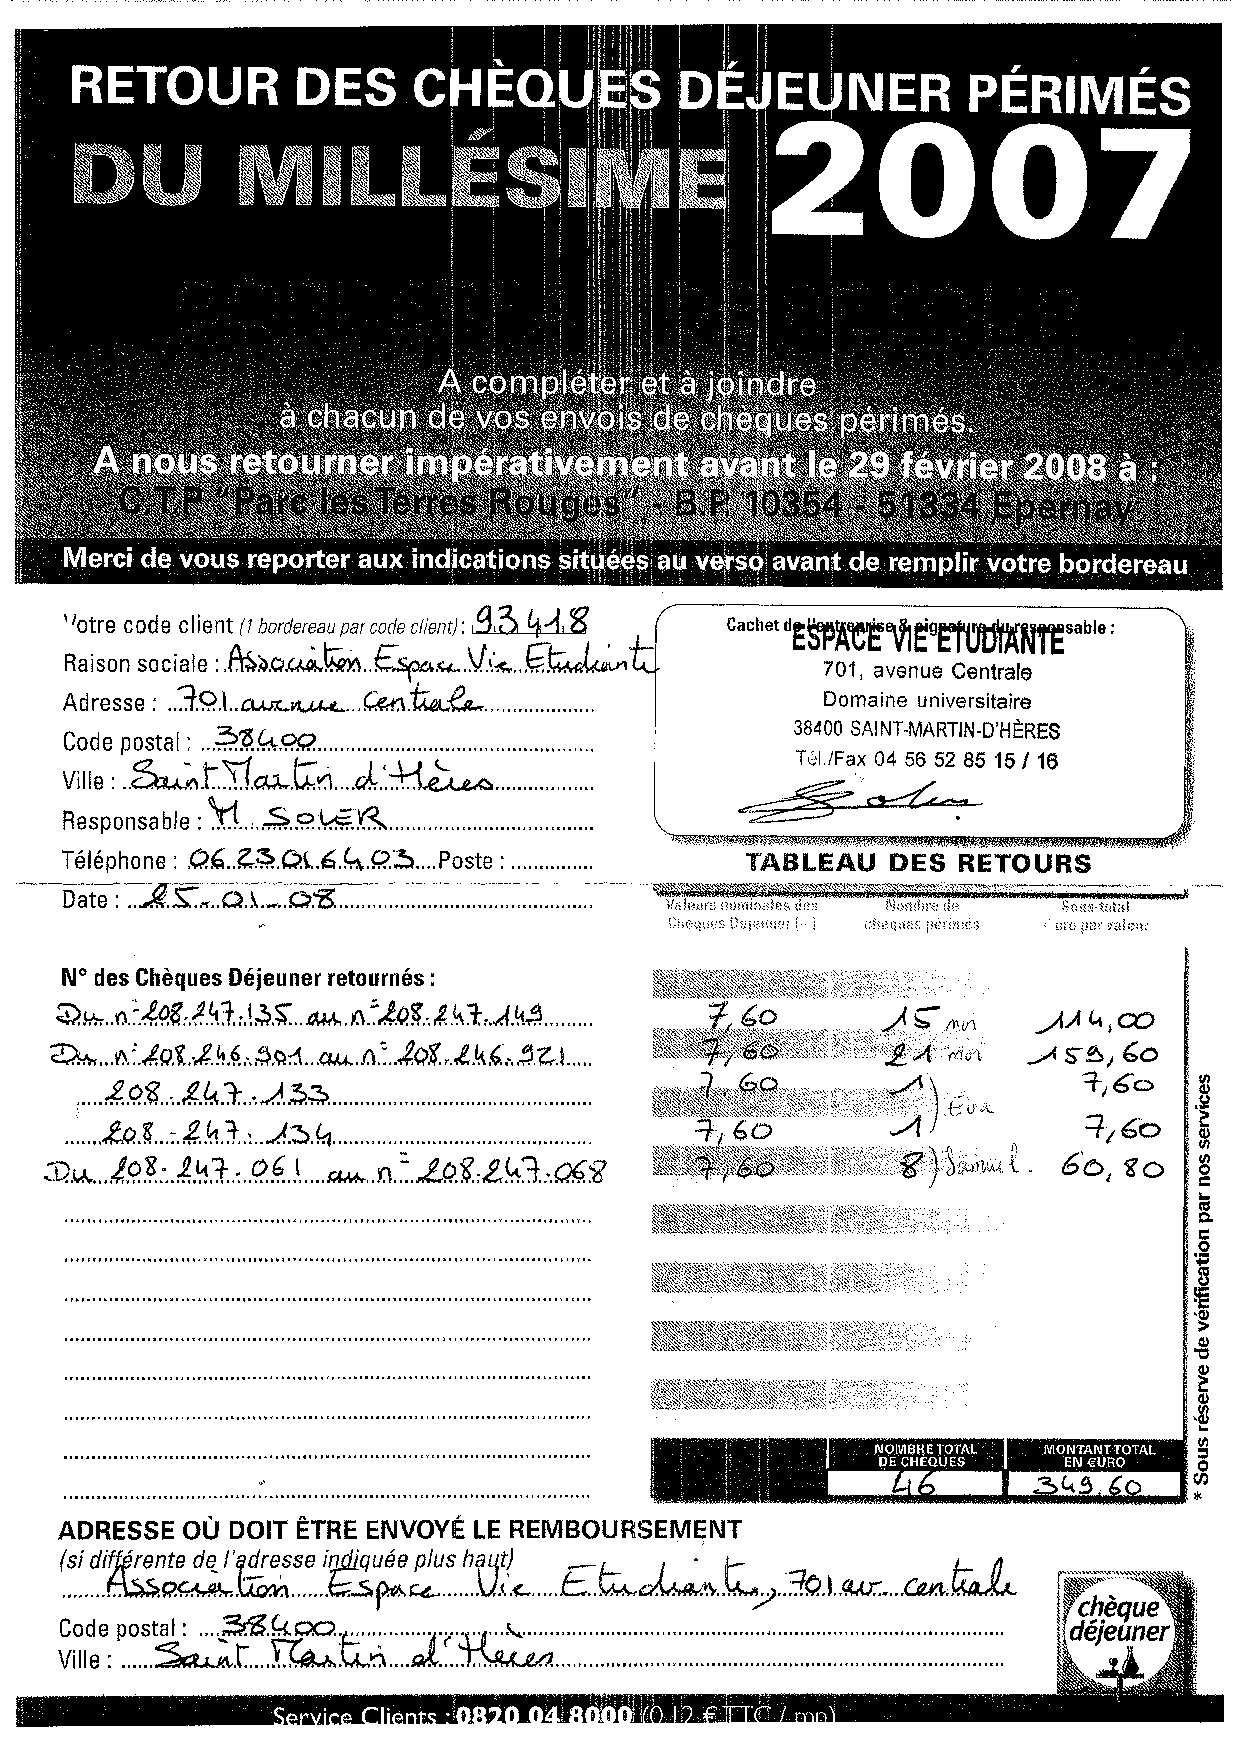
\includegraphics[scale=0.7]{annexes/images/chequedejeuner_retour.pdf}
\end{center}


\subsection{Exemple de facture client : DSI}
\begin{center}
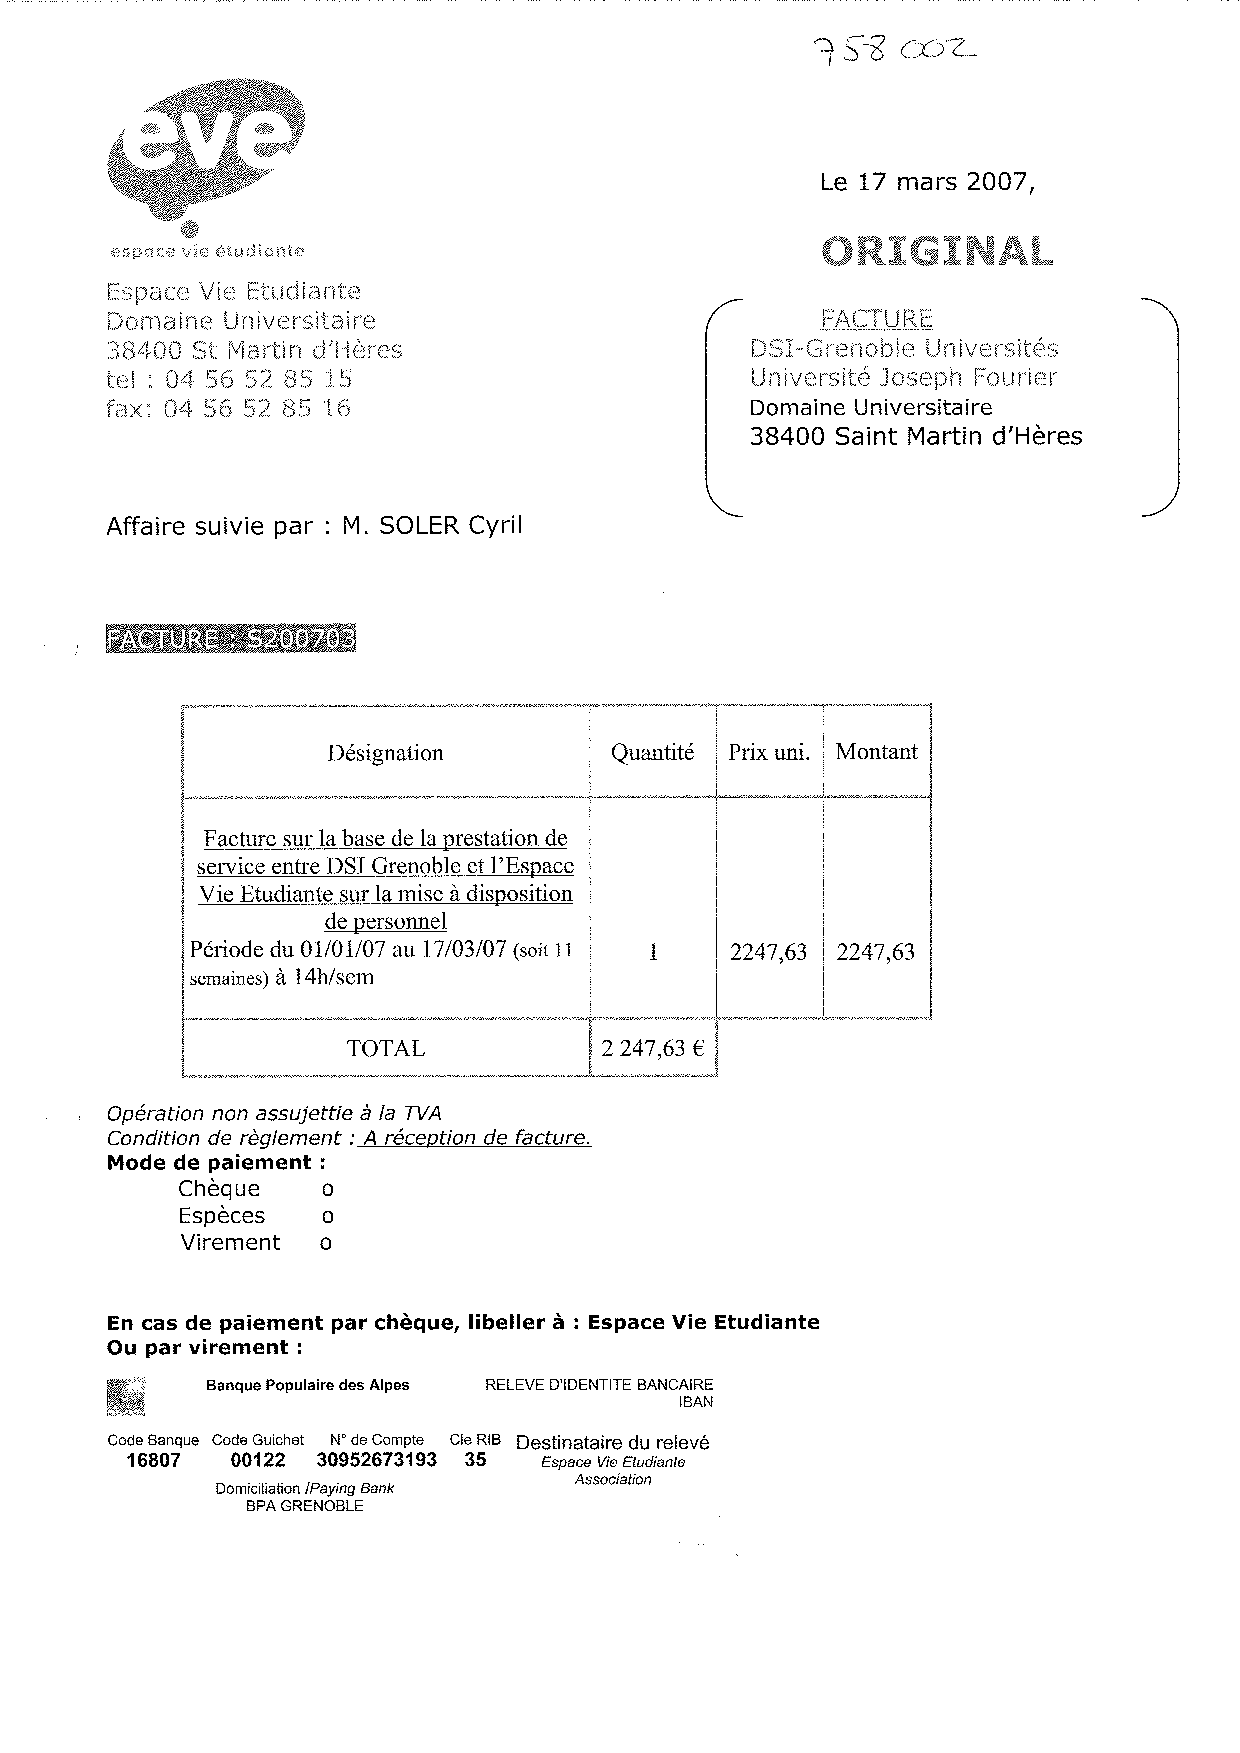
\includegraphics[scale=0.7]{annexes/images/facture_client_dsi.pdf}
\end{center}
\subsection{Exemple de facture client : UJF}
\begin{center}
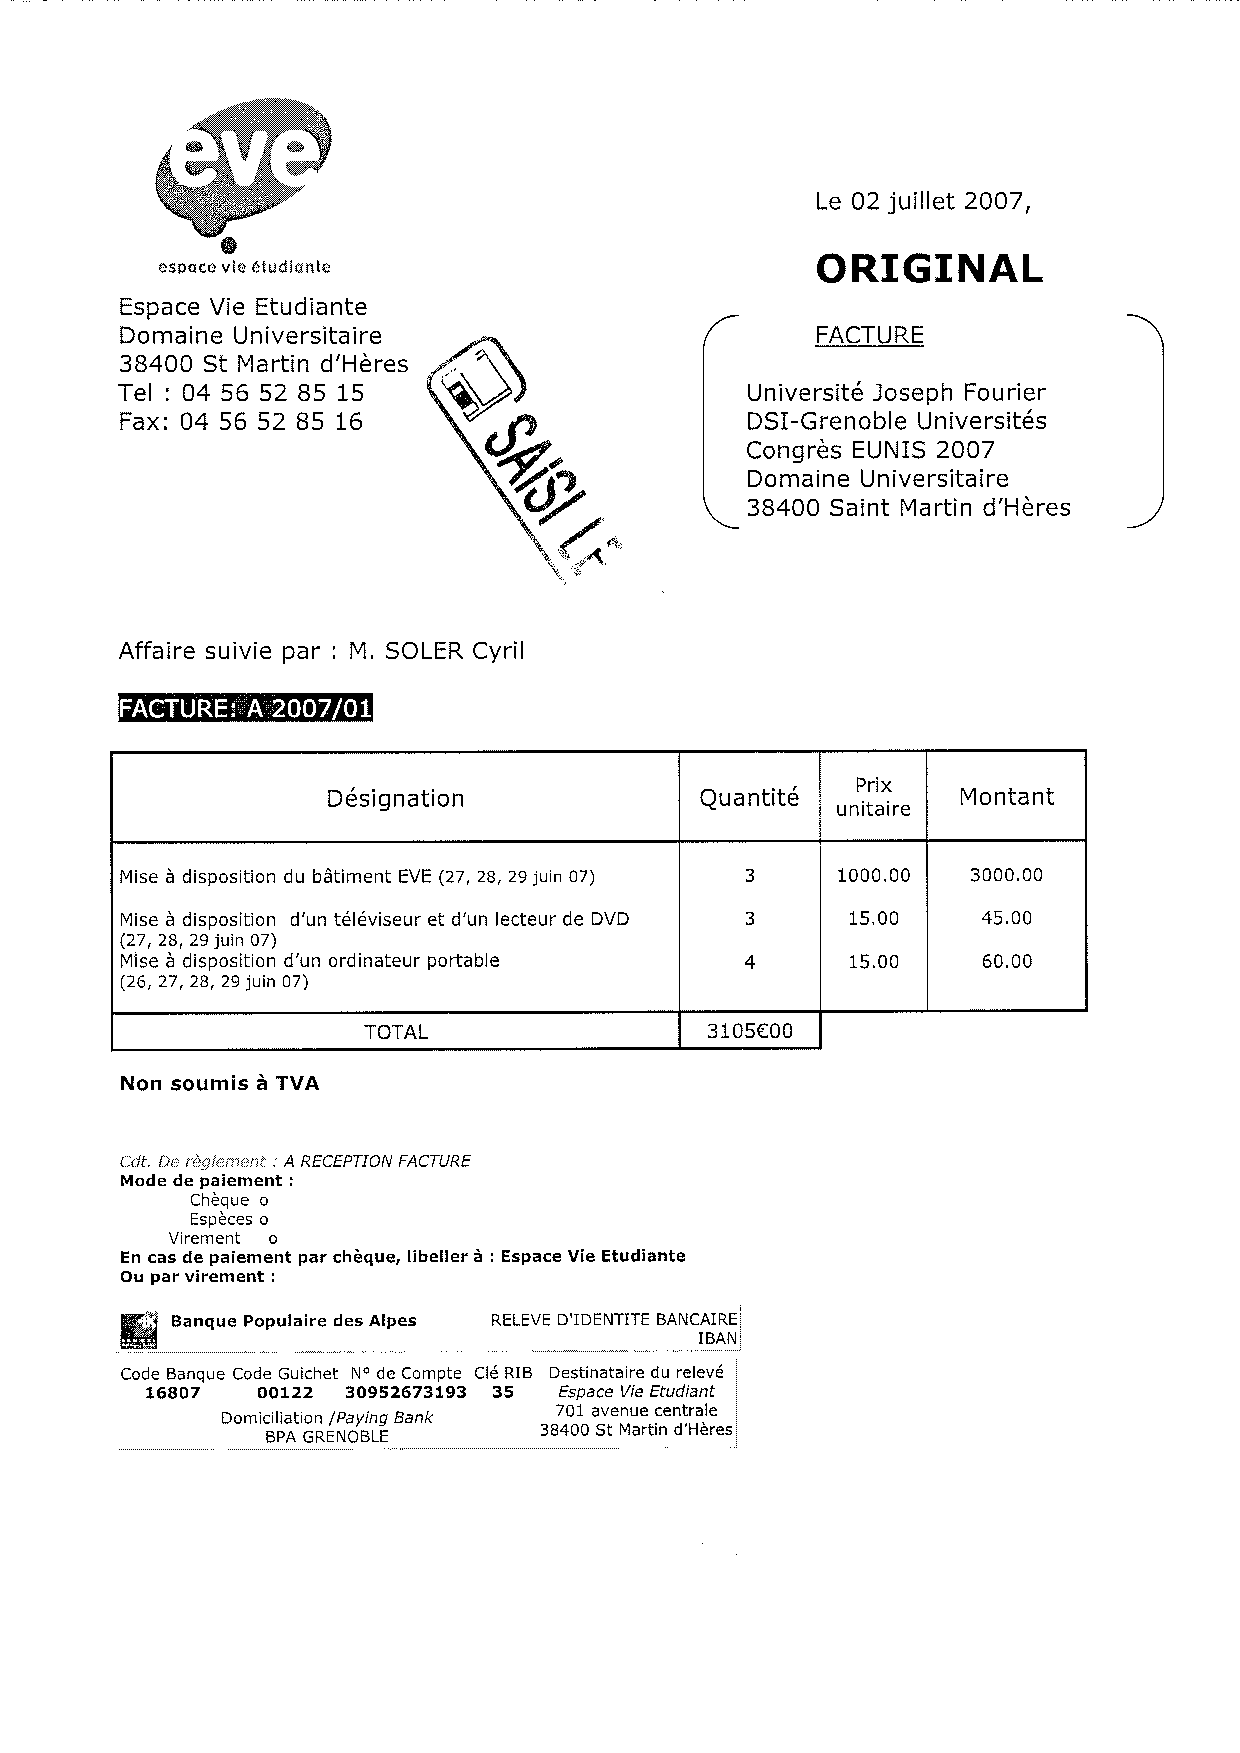
\includegraphics[scale=0.7]{annexes/images/facture_client_mise_a_disposition.pdf}
\end{center}

%\subsection{titre}
%\begin{center}
%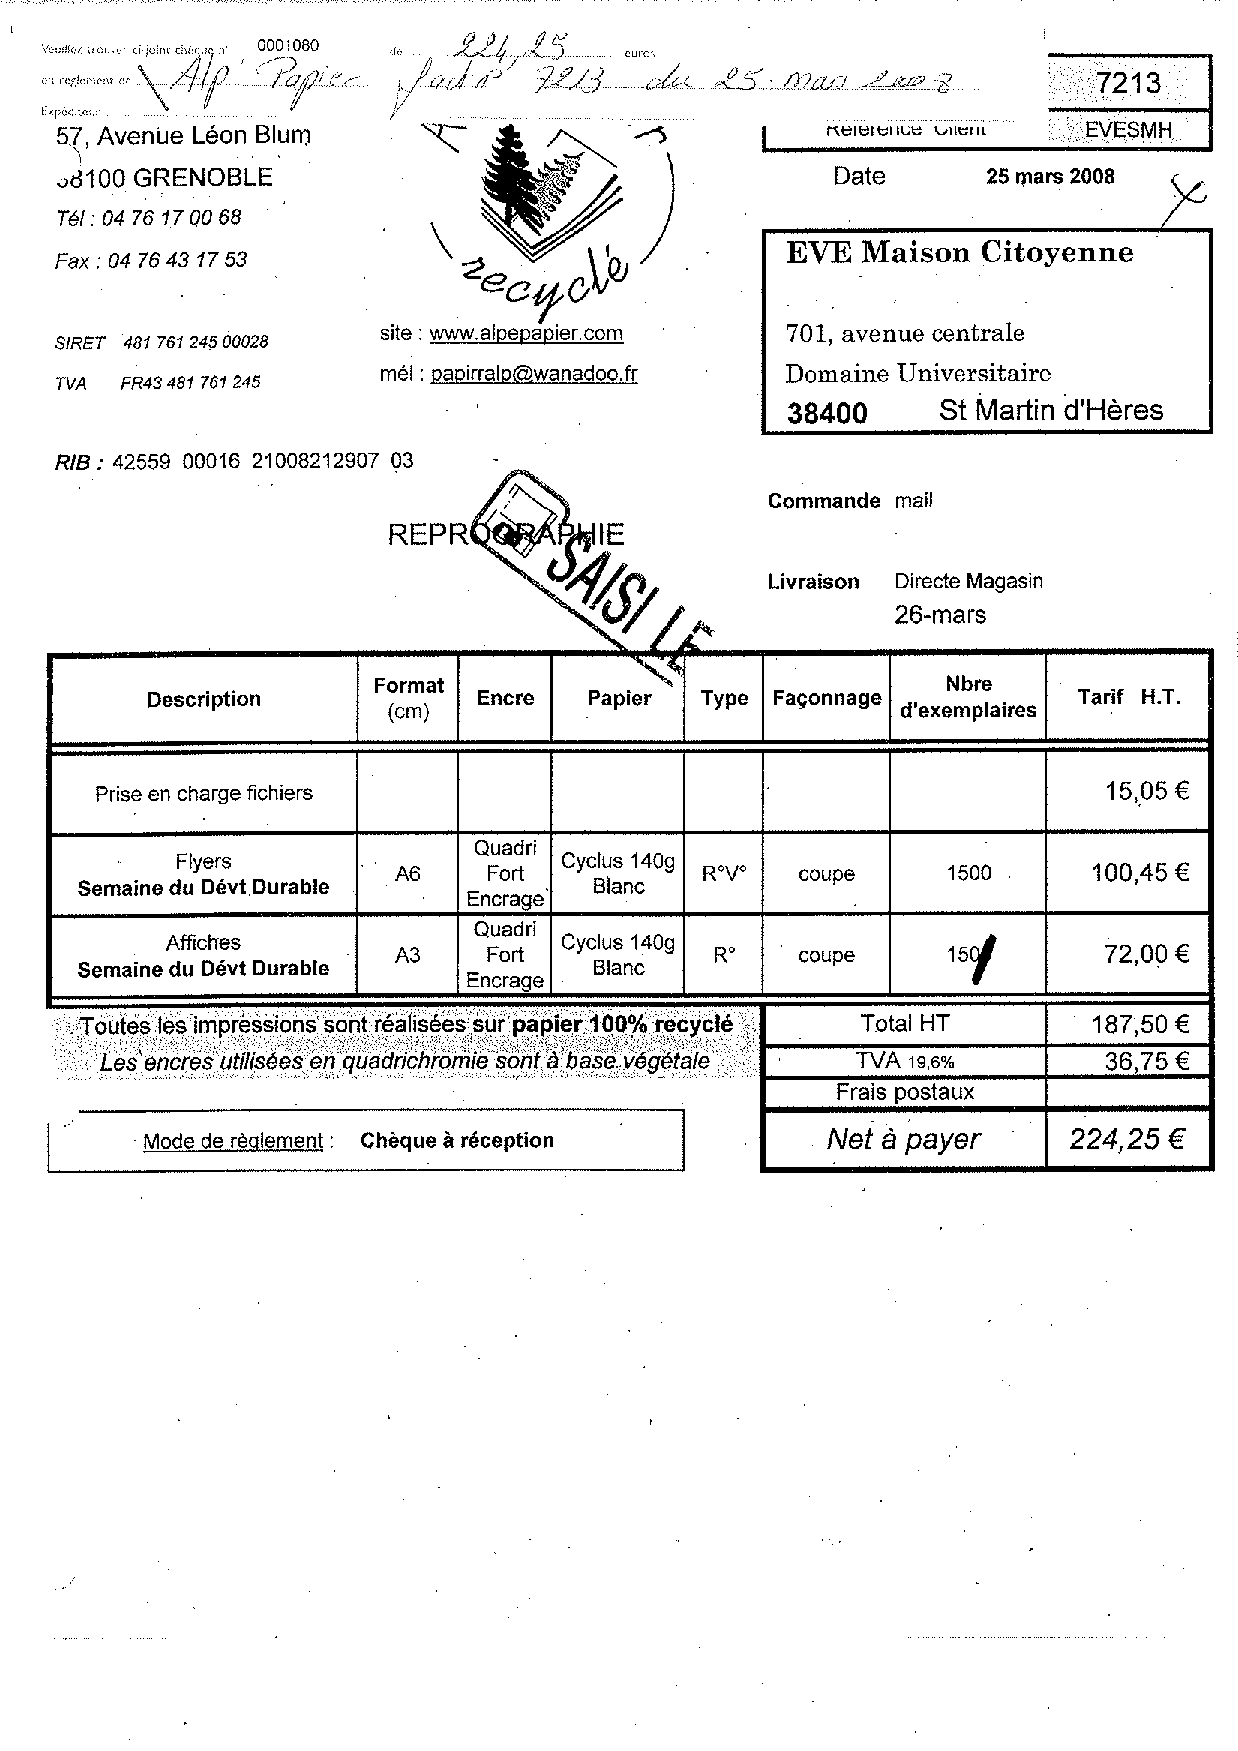
\includegraphics[scale=0.6]{annexes/images/facture_fournisseur_repro.pdf}
%\end{center}
\subsection{Contrats d'avenir : coûts indicatifs}
\begin{center}
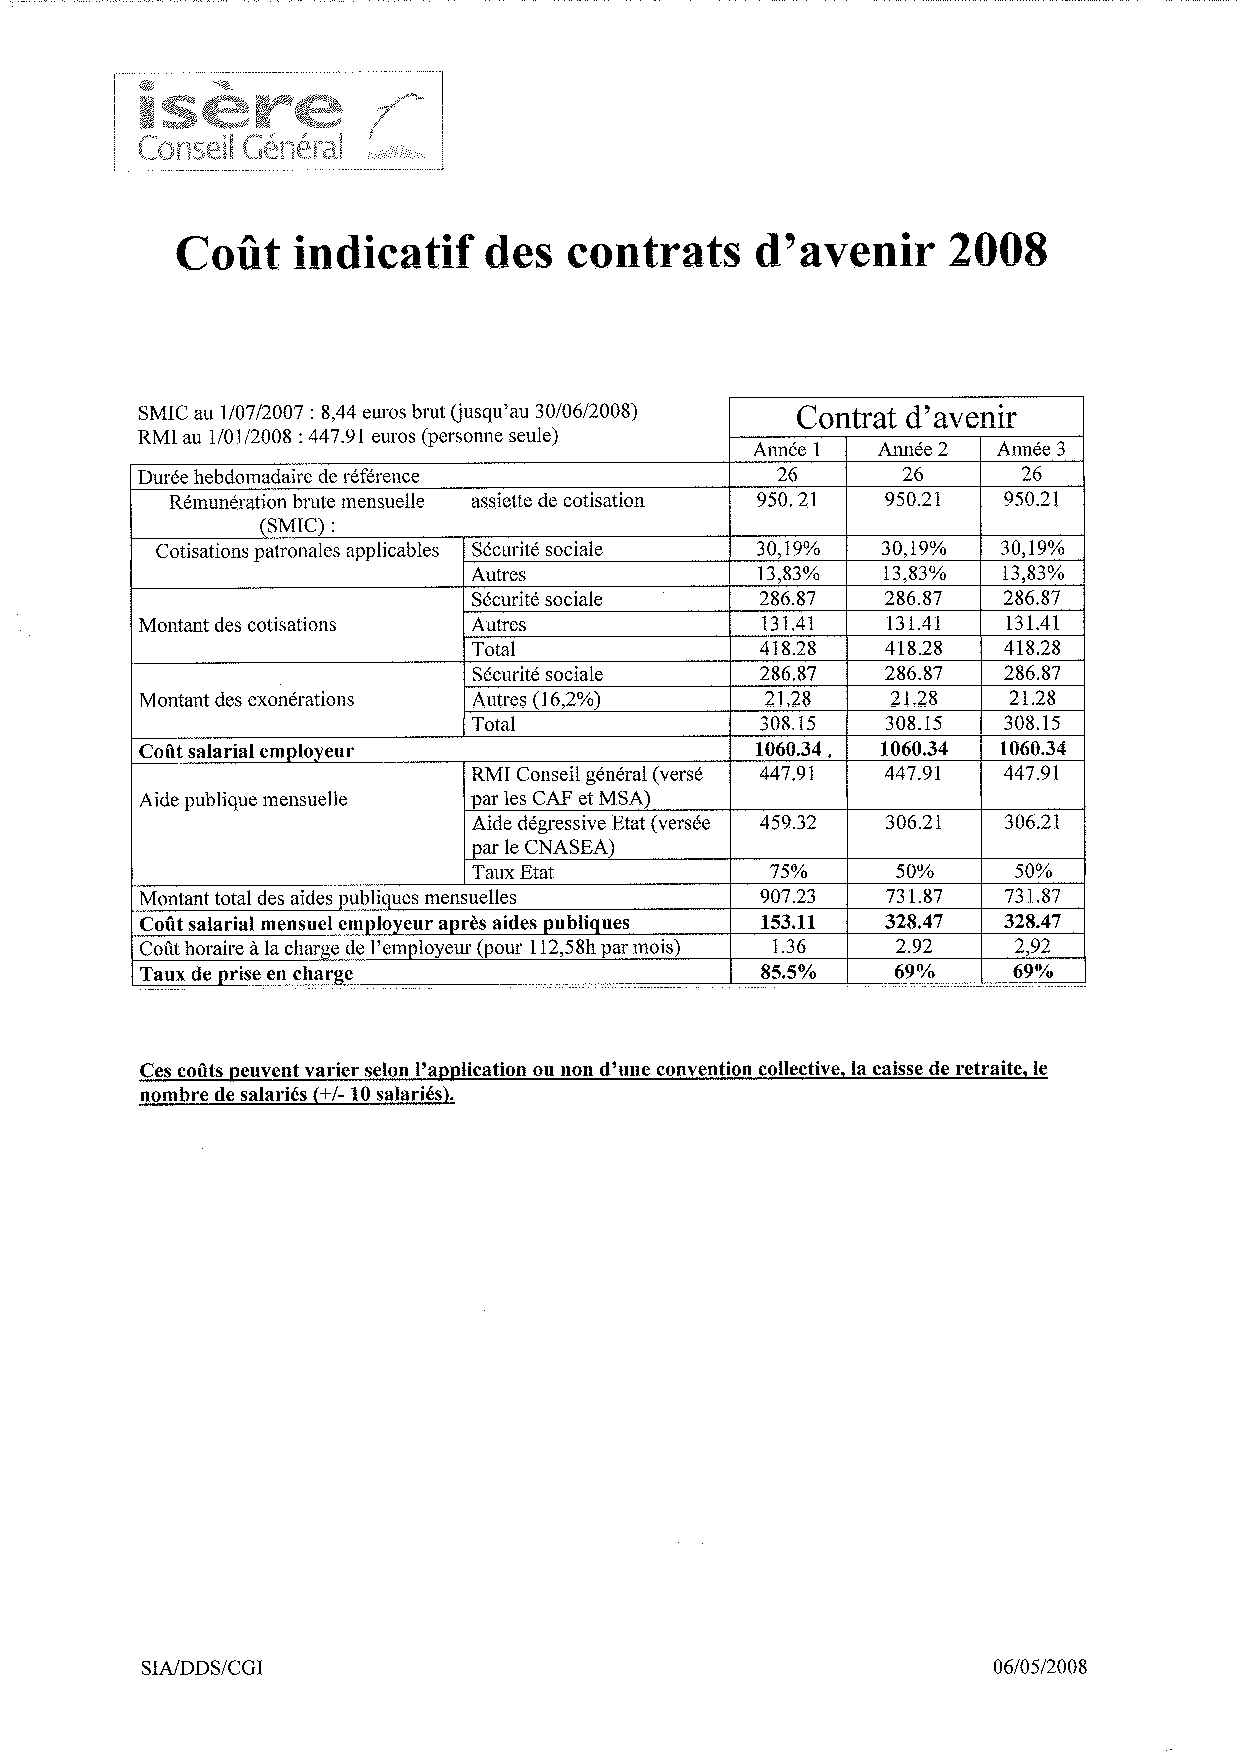
\includegraphics[scale=0.7]{annexes/images/contrats_avenir_indicatif.pdf}
\end{center}
\subsection{Exemple de fiche de paie}
\begin{center}
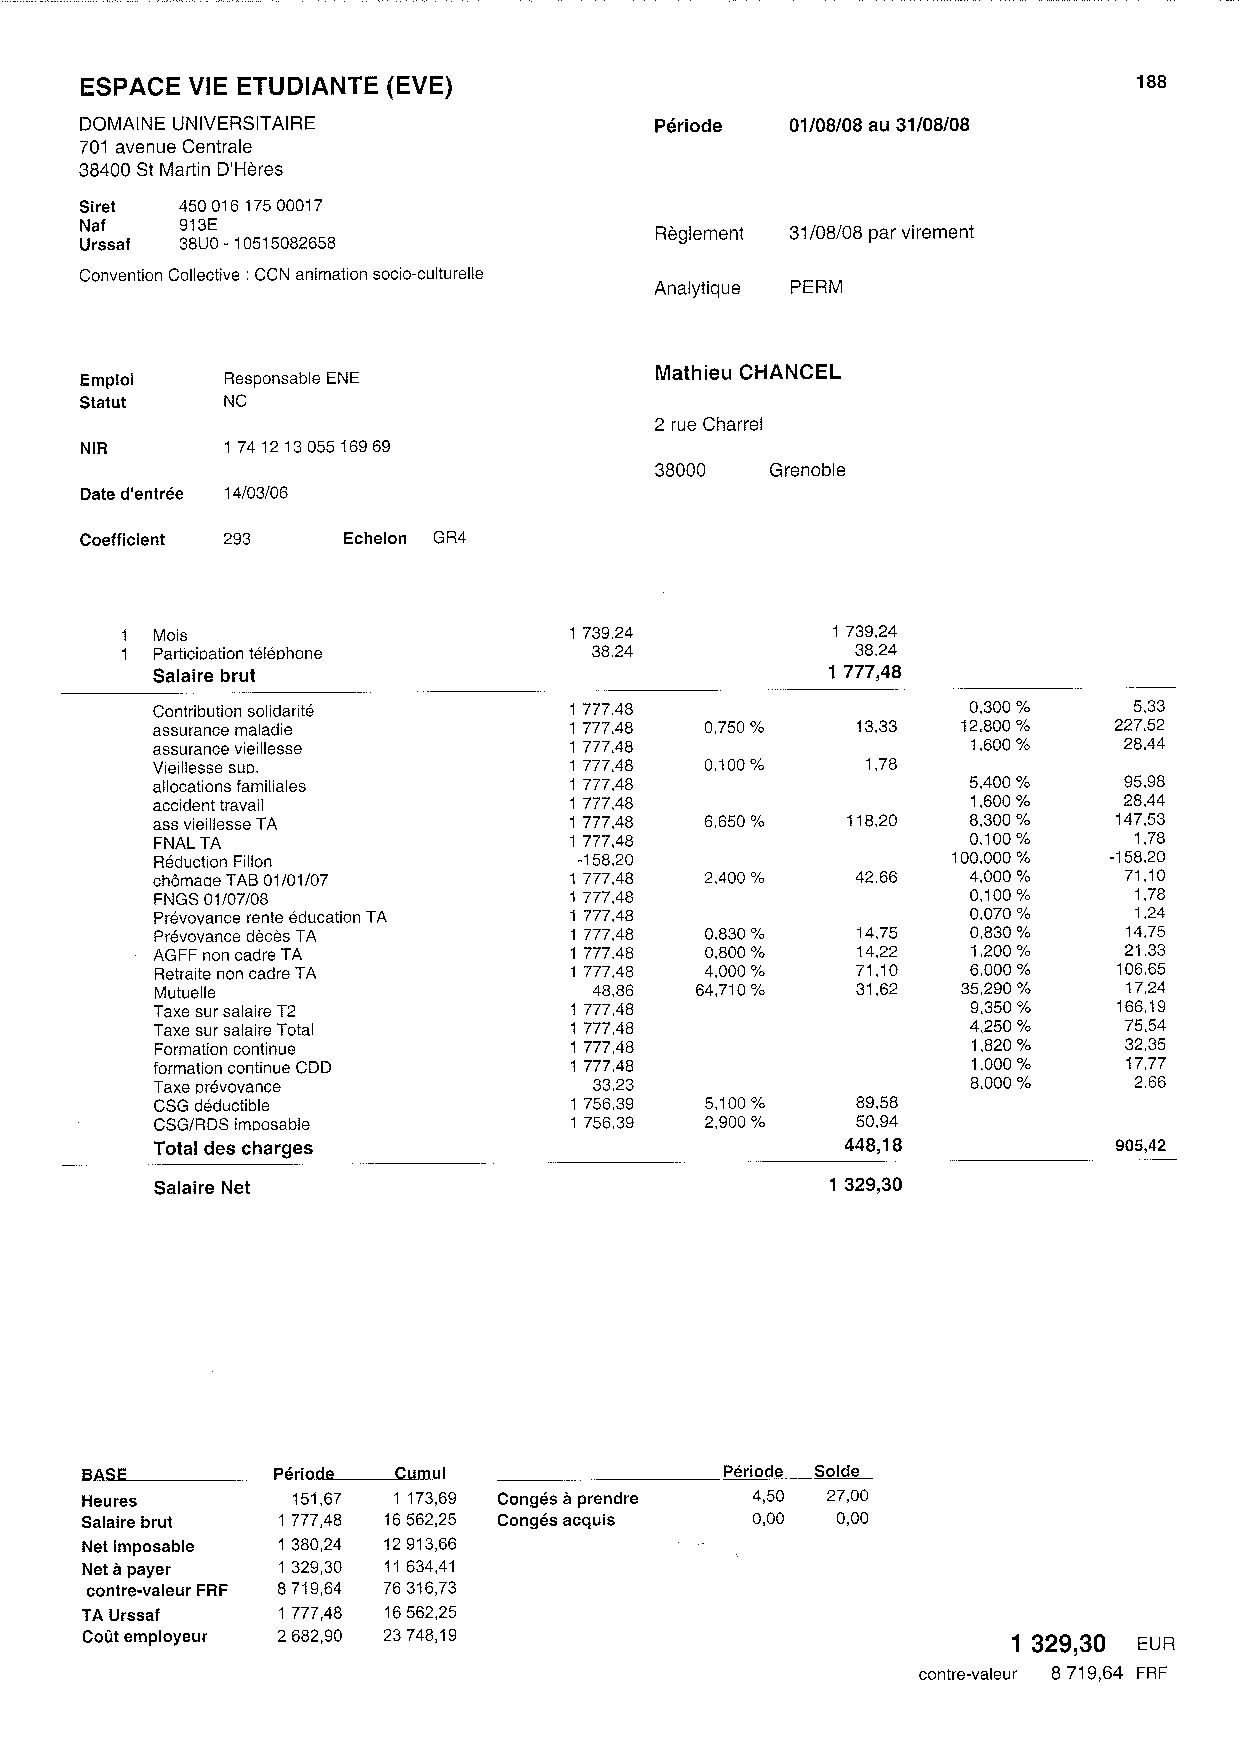
\includegraphics[scale=0.7]{annexes/images/fiche_paye_mat.pdf}
\end{center}



\section{Délégation de Service Public}

La compréhension des contrats et conventions régissant le fonctionnement d'une
structure nous apparait comme indispensable pour l'appréhension des limites de
flexibilité de ses règles de gestion. Nous nous sommes donc attachés à l'analyse
de la Délégation de Service Public, présente ci-dessous, et de la convention
de l'Assistance Informatique, que nous n'exposerons pas puisqu'elle expirera 
définitivement en décembre 2008.

\newpage

\begin{center}
	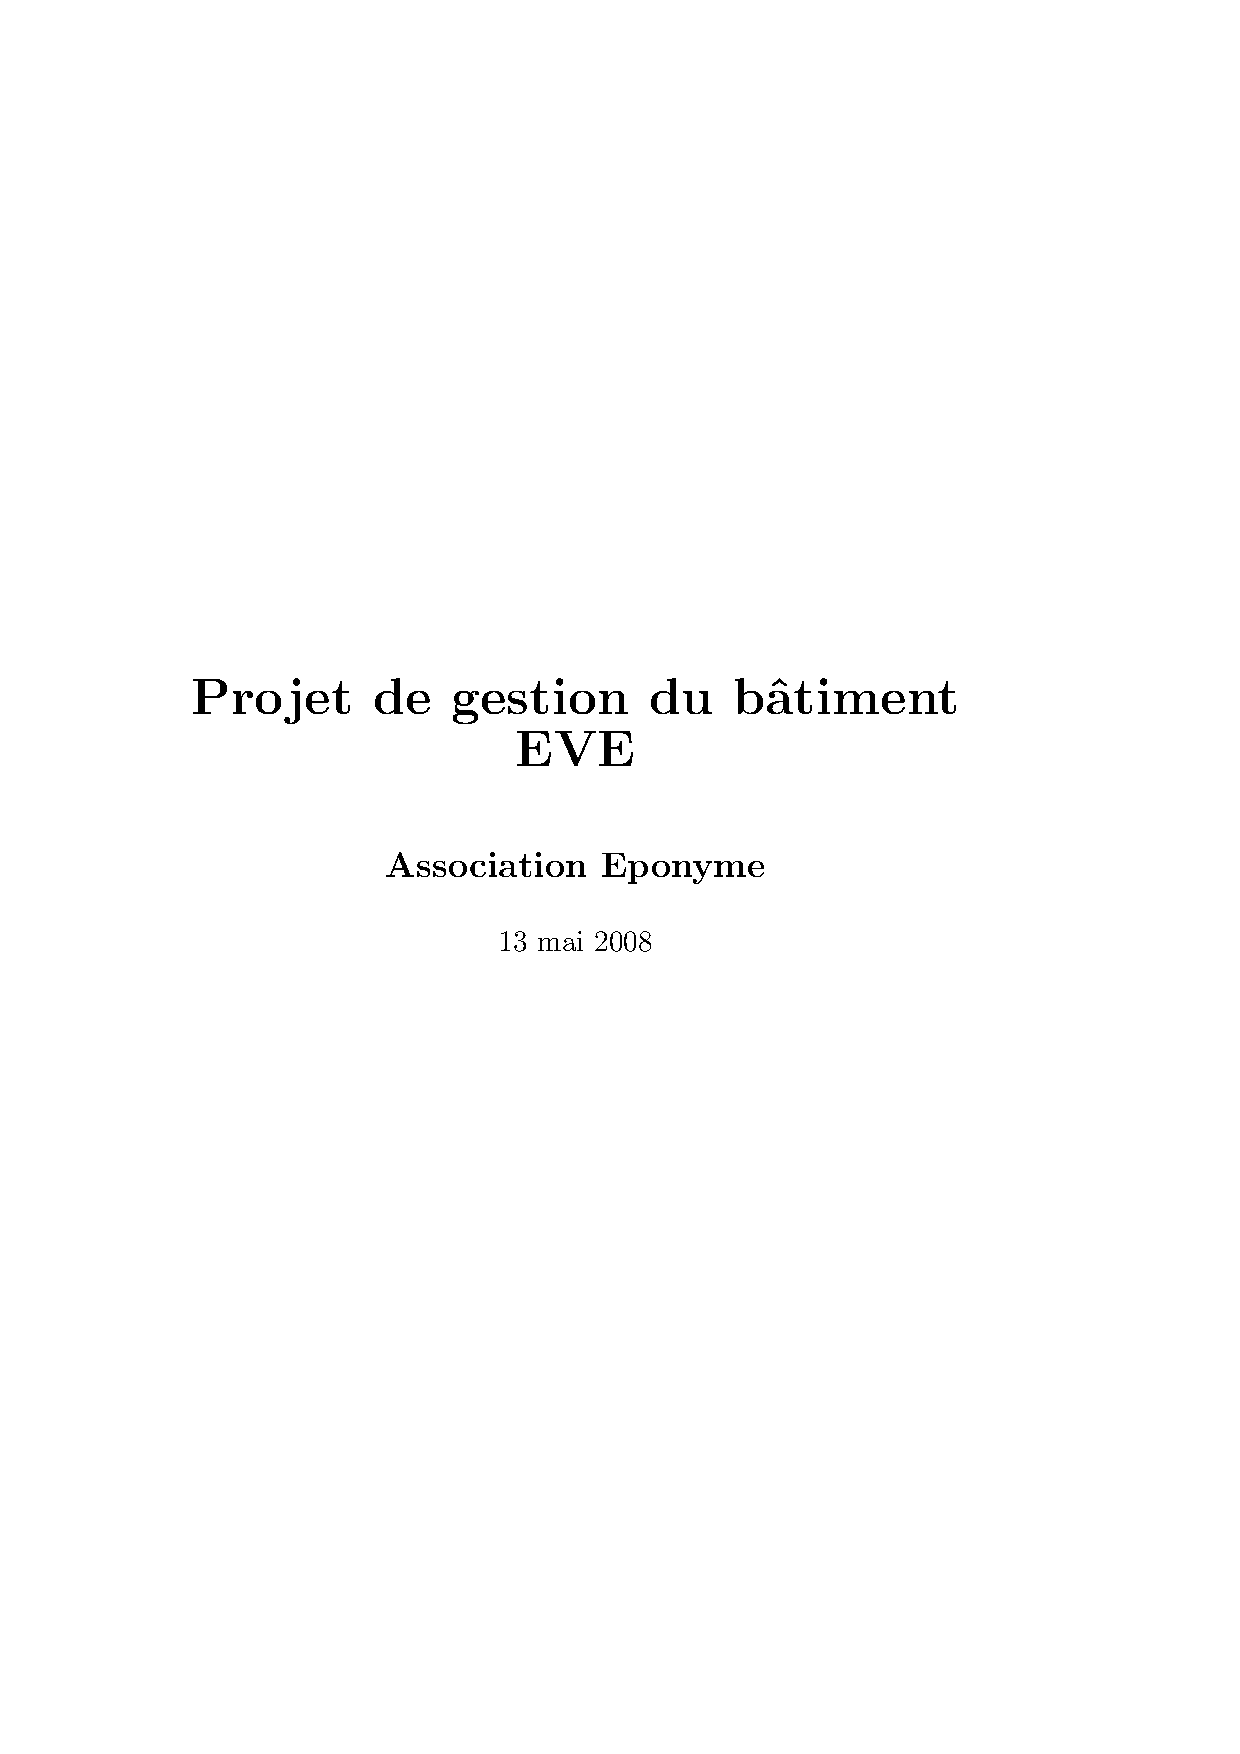
\includegraphics[scale=0.85,trim=20mm 20mm 20mm 20mm,clip,page=1]{annexes/candidature_dsp.pdf} \\
Dossier de candidature DSP, page 1
\newpage
\includegraphics[scale=0.85,trim=20mm 20mm 20mm 20mm,clip,page=2]{annexes/candidature_dsp.pdf} \\
Dossier de candidature DSP, page 2
\newpage
\includegraphics[scale=0.85,trim=20mm 20mm 20mm 20mm,clip,page=3]{annexes/candidature_dsp.pdf} \\
Dossier de candidature DSP, page 3
\newpage
\includegraphics[scale=0.85,trim=20mm 20mm 20mm 20mm,clip,page=4]{annexes/candidature_dsp.pdf} \\
Dossier de candidature DSP, page 4
\newpage
\includegraphics[scale=0.85,trim=20mm 20mm 20mm 20mm,clip,page=5]{annexes/candidature_dsp.pdf} \\
Dossier de candidature DSP, page 5
\newpage
\includegraphics[scale=0.85,trim=20mm 20mm 20mm 20mm,clip,page=6]{annexes/candidature_dsp.pdf} \\
Dossier de candidature DSP, page 6
\newpage
\includegraphics[scale=0.85,trim=20mm 20mm 20mm 20mm,clip,page=7]{annexes/candidature_dsp.pdf} \\
Dossier de candidature DSP, page 7
\newpage
\includegraphics[scale=0.85,trim=20mm 20mm 20mm 20mm,clip,page=8]{annexes/candidature_dsp.pdf} \\
Dossier de candidature DSP, page 8
\newpage
\includegraphics[scale=0.85,trim=20mm 20mm 20mm 20mm,clip,page=9]{annexes/candidature_dsp.pdf} \\
Dossier de candidature DSP, page 9
\newpage
\includegraphics[scale=0.85,trim=20mm 20mm 20mm 20mm,clip,page=10]{annexes/candidature_dsp.pdf} \\
Dossier de candidature DSP, page 10
\newpage
\includegraphics[scale=0.85,trim=20mm 20mm 20mm 20mm,clip,page=11]{annexes/candidature_dsp.pdf} \\
Dossier de candidature DSP, page 11
\newpage
\includegraphics[scale=0.85,trim=20mm 20mm 20mm 20mm,clip,page=12]{annexes/candidature_dsp.pdf} \\
Dossier de candidature DSP, page 12
\newpage
\includegraphics[scale=0.85,trim=20mm 20mm 20mm 20mm,clip,page=13]{annexes/candidature_dsp.pdf} \\
Dossier de candidature DSP, page 13
\newpage
\includegraphics[scale=0.85,trim=20mm 20mm 20mm 20mm,clip,page=14]{annexes/candidature_dsp.pdf} \\
Dossier de candidature DSP, page 14
\newpage
\includegraphics[scale=0.85,trim=20mm 20mm 20mm 20mm,clip,page=15]{annexes/candidature_dsp.pdf} \\
Dossier de candidature DSP, page 15
\newpage
\includegraphics[scale=0.85,trim=20mm 20mm 20mm 20mm,clip,page=16]{annexes/candidature_dsp.pdf} \\
Dossier de candidature DSP, page 16
\newpage
\includegraphics[scale=0.85,trim=20mm 20mm 20mm 20mm,clip,page=17]{annexes/candidature_dsp.pdf} \\
Dossier de candidature DSP, page 17
\newpage
\includegraphics[scale=0.85,trim=20mm 20mm 20mm 20mm,clip,page=18]{annexes/candidature_dsp.pdf} \\
Dossier de candidature DSP, page 18
\newpage
\includegraphics[scale=0.85,trim=20mm 20mm 20mm 20mm,clip,page=19]{annexes/candidature_dsp.pdf} \\
Dossier de candidature DSP, page 19
\newpage
\includegraphics[scale=0.85,trim=20mm 20mm 20mm 20mm,clip,page=20]{annexes/candidature_dsp.pdf} \\
Dossier de candidature DSP, page 20
\newpage
\includegraphics[scale=0.85,trim=20mm 20mm 20mm 20mm,clip,page=21]{annexes/candidature_dsp.pdf} \\
Dossier de candidature DSP, page 21
\newpage
\includegraphics[scale=0.85,trim=20mm 20mm 20mm 20mm,clip,page=22]{annexes/candidature_dsp.pdf} \\
Dossier de candidature DSP, page 22
\newpage
\includegraphics[scale=0.85,trim=20mm 20mm 20mm 20mm,clip,page=23]{annexes/candidature_dsp.pdf} \\
Dossier de candidature DSP, page 23
\newpage
\includegraphics[scale=0.85,trim=20mm 20mm 20mm 20mm,clip,page=24]{annexes/candidature_dsp.pdf} \\
Dossier de candidature DSP, page 24
\newpage
\includegraphics[scale=0.85,trim=20mm 20mm 20mm 20mm,clip,page=25]{annexes/candidature_dsp.pdf} \\
Dossier de candidature DSP, page 25
\newpage
\includegraphics[scale=0.85,trim=20mm 20mm 20mm 20mm,clip,page=26]{annexes/candidature_dsp.pdf} \\
Dossier de candidature DSP, page 26
\newpage
\includegraphics[scale=0.85,trim=20mm 20mm 20mm 20mm,clip,page=27]{annexes/candidature_dsp.pdf} \\
Dossier de candidature DSP, page 27
\newpage
\includegraphics[scale=0.85,trim=20mm 20mm 20mm 20mm,clip,page=28]{annexes/candidature_dsp.pdf} \\
Dossier de candidature DSP, page 28
\newpage
\includegraphics[scale=0.85,trim=20mm 20mm 20mm 20mm,clip,page=29]{annexes/candidature_dsp.pdf} \\
Dossier de candidature DSP, page 29
\newpage
\includegraphics[scale=0.85,trim=20mm 20mm 20mm 20mm,clip,page=30]{annexes/candidature_dsp.pdf} \\
Dossier de candidature DSP, page 30
\newpage
\includegraphics[scale=0.85,trim=20mm 20mm 20mm 20mm,clip,page=31]{annexes/candidature_dsp.pdf} \\
Dossier de candidature DSP, page 31
\newpage
\includegraphics[scale=0.85,trim=20mm 20mm 20mm 20mm,clip,page=32]{annexes/candidature_dsp.pdf} \\
Dossier de candidature DSP, page 32
\newpage
\includegraphics[scale=0.85,trim=20mm 20mm 20mm 20mm,clip,page=33]{annexes/candidature_dsp.pdf} \\
Dossier de candidature DSP, page 33
\newpage
\includegraphics[scale=0.85,trim=20mm 20mm 20mm 20mm,clip,page=34]{annexes/candidature_dsp.pdf} \\
Dossier de candidature DSP, page 34
\newpage
\includegraphics[scale=0.85,trim=20mm 20mm 20mm 20mm,clip,page=35]{annexes/candidature_dsp.pdf} \\
Dossier de candidature DSP, page 35
\newpage
\includegraphics[scale=0.85,trim=20mm 20mm 20mm 20mm,clip,page=36]{annexes/candidature_dsp.pdf} \\
Dossier de candidature DSP, page 36
\newpage
\includegraphics[scale=0.85,trim=20mm 20mm 20mm 20mm,clip,page=37]{annexes/candidature_dsp.pdf} \\
Dossier de candidature DSP, page 37
\newpage
\includegraphics[scale=0.85,trim=20mm 20mm 20mm 20mm,clip,page=38]{annexes/candidature_dsp.pdf} \\
Dossier de candidature DSP, page 38
\newpage
\includegraphics[scale=0.85,trim=20mm 20mm 20mm 20mm,clip,page=39]{annexes/candidature_dsp.pdf} \\
Dossier de candidature DSP, page 39
\newpage
\includegraphics[scale=0.85,trim=20mm 20mm 20mm 20mm,clip,page=40]{annexes/candidature_dsp.pdf} \\
Dossier de candidature DSP, page 40
\newpage
\includegraphics[scale=0.85,trim=20mm 20mm 20mm 20mm,clip,page=41]{annexes/candidature_dsp.pdf} \\
Dossier de candidature DSP, page 41
\newpage
\includegraphics[scale=0.85,trim=20mm 20mm 20mm 20mm,clip,page=42]{annexes/candidature_dsp.pdf} \\
Dossier de candidature DSP, page 42
\newpage
\includegraphics[scale=0.85,trim=20mm 20mm 20mm 20mm,clip,page=43]{annexes/candidature_dsp.pdf} \\
Dossier de candidature DSP, page 43
\newpage
\includegraphics[scale=0.85,trim=20mm 20mm 20mm 20mm,clip,page=44]{annexes/candidature_dsp.pdf} \\
Dossier de candidature DSP, page 44
\newpage

\end{center}

\newpage

\subsection{Références}

\begin{itemize}
\item \textbf{Site Web de EVE}, \textit{http://www.eve-grenoble.org/}
\item \textbf{EBP}, \textit{http://www.ebp.com/fr/}
\item \textbf{Orchestra Software}, \textit{http://www.orchestra-software.com/}
\item \textbf{phpMyAdmin}, \textit{http://www.phpmyadmin.net/}
\end{itemize}

\section*{Remerciements}

Nous remercions l'ensemble de EVE, en particulier Claire Guichoux, David Rouquet,
Olivier Royer, Samuel Chopin pour leur transparence et le temps qu'ils ont pu
nous accorder, Jean-Michel Spinard pour nous offrir l'opportunité d'aborder
la problématique des SI au sein des organisations,
Maïna Le Poul pour son hospitalité, Noémie Verzat pour sa patience et
les auteurs de Graphviz et \LaTeXe pour l'efficacité de leur outils.